% $Id$
% Author: Dave Fournier
% Copyright (c) 2008 Regents of the University of California


\documentclass{admbmanual}
\makeatletter\@twosidefalse\makeatother
\hypersetup{urlcolor=black}

% Some local definitions.
\newcommand\mybackslash{$\backslash$}
\newcommand\bmax{B_{\textrm{MAX}}}
\newcommand\DS{\texttt{DATA\_SECTION}}
\newcommand\RS{\texttt{REPORT\_SECTION}}
\newcommand\PS{\texttt{PARAMETER\_SECTION}}
\newcommand\PCS{\texttt{PRELIMINARY\_CALCS\_SECTION}}
\newcommand\IS{\texttt{INITIALIZATION\_SECTION}}
\newcommand\PROS{\texttt{PROCEDURE\_SECTION}}
\newcommand\apl{profile likelihood}
\newcommand{\cobs}{C^{obs}_i}
%\newcommand\ls{least-squares }
%\newcommand\ei{\epsilon_i}
%\newcommand\mm{least median of squared residuals }
%\newcommand\pr{{\bf[P]}}
\newcommand\aone{a_{t|t-1}}
\newcommand\Pone{P_{t|t-1}}
\newcommand\diag{\textrm{diag}}
\newcommand\ep{\textrm{elem\_prod}}

\makeindex

\begin{document}

\title{%
  \smalltitlepart{An Introduction to}
  \largetitlepart{AD MODEL BUILDER}
  \smalltitlepart{for Use in Nonlinear Modeling and Statistics}
  \vspace{3ex}\textsf{\textit{Version 10.0~~(2011-01-18)}}\vspace{3ex}
}
\author{\textsf{\textit{David Fournier}}}
\manualname{AD Model Builder}
\maketitle
%%xx \htmlnewfile

~\vfill
\noindent ADMB Foundation, Honolulu.\\\\
\noindent This is the manual for AD Model Builder (ADMB) version 10.0.\\\\
\noindent Copyright \copyright\ 1993, 1994, 1996, 2000, 2001, 2004, 2007, 2008,
2011 David Fournier\\\\
\noindent The latest edition of the manual is available at:\\
\url{http://admb-project.org/documentation/manuals/admb-user-manuals}

\tableofcontents

\chapter{Getting Started with \ADM}

This manual describes \ADM, the fastest, most powerful software for rapid
development and fitting of general nonlinear statistical models available. The
accompanying demonstration disk has a number of example programs from various
fields, including chemical engineering, natural resource modeling, and financial
modeling. As you will see, with a few statements, you can build powerful
programs to solve problems that would completely defeat other modeling
environments. The \ADM\ environment makes it simple to deal with recurring
difficulties in nonlinear modeling, such as restricting the values that
parameters can assume, carrying out the optimization in a stepwise manner, and
producing a report of the estimates of the standard deviations of the parameter
estimates. In addition, these techniques scale up to models with at least 5000
independent parameters on a 1000 MHz Pentium III, and more on more powerful
platforms. So, if you are interested in a really powerful environment for
nonlinear modeling---read on!
\X{template}
\X{default behavior}

\ADM\ provides a template-like approach to code generation. Instead of needing
to write all the code for the model, the user can employ any \textsc{ascii} file
editor to simply fill in the template, describing the particular aspects of the
model---data, model parameters, and the fitting criterion---to be used. With
this approach, the specification of the model is reduced to the absolute minimum
number of statements. Reasonable default behavior for various aspects of
modeling, such as the input of data and initial parameters, and reporting of
results, are provided. Of course, it is possible to override this default
behavior to customize an application when desired. The command line argument
\texttt{-ind NAME} followed by the string \texttt{NAME} changes the default data
input file to \texttt{NAME}, where \texttt{NAME} is any name you~like.
\XX{command line arguments}{\fontindexentry{tt}{-ind NAME input data file}}

The various concepts embodied in \ADM\ are introduced in a series of examples.
You should at least skim through each of the examples in the order they appear,
so that you will be familiar with the concepts used in the later examples. The
examples disk contains the \ADM\ template code, the \cplus\ code produced by
\ADM, and the executable programs produced by compiling the \cplus\ code. This
process of producing the executable is automated, so that the user who doesn't
wish to consider the vagaries of \cplus\ programming can go from the \ADM\
template to the compiled executable in one step. Assuming that the \cplus\
compiler and the \ADM\ and \scAD\ libraries have been properly installed, then
to produce a \ADM\ executable, it is only necessary to type \texttt{makeadm
  root}, where \texttt{root.tpl} is the name of the \textsc{ascii} file
containing the template specification. To simplify model development, two modes
of operation are provided: a safe mode with bounds checking on all array
objects, and an optimized mode, for fastest execution.

\X{automatic differentiation}
\X{adjoint code}
\ADM\ achieves its high performance levels by employing the \scAD\ \cplus\ class
library. \scAD\ combines an array language with the reverse mode of automatic
differentiation, supplemented with precompiled adjoint code for the derivatives
of common array and matrix operations. However, all of this is completely
transparent to the \ADM\ user. It is only necessary to provide a simple
description of the statistical model desired, and the entire process of fitting
the model to data and reporting the results is taken care of automatically.

Although \cplus\ potentially provides good support for mathematical modeling,
the language is rather complex---it cannot be learned in a few days. Moreover,
many features of the language are not needed for mathematical modeling. A novice
user who wishes to build mathematical models may have a difficult time deciding
what features of the language to learn and what features can be ignored until
later. \ADM\ is intended to help overcome these difficulties and to speed up
model development. When using \ADM, most of the aspects of \cplus\ programming
are hidden from the user. In fact, the beginning user can be almost unaware that
\cplus\ underlies the implementation of \ADM. It is only necessary to be
familiar with some of the simpler aspects of C or \cplus~syntax.

\XX{Markov chain simulation}{Hastings-Metropolis algorithm}
\XX{Markov chain simulation}{to estimate the posterior distribution}
\X{Hastings-Metropolis algorithm}
To interpret the results of the statistical analysis, \ADM\ provides simple
methods for calculating the profile likelihood and Markov chain simulation
estimates of the posterior distribution for parameters of interest
(Hastings-Metropolis algorithm).

\section{What are nonlinear statistical models?}

\ADMS is software for creating computer programs to estimate the parameters (or
the probability distribution of parameters) for nonlinear statistical models.
This raises the question: ``What is a nonlinear statistical model?'' Consider
the following model. We have a set of observations $Y_i$ and $x_{ij}$, where it
is assumed that
\begin{equation}
{Y_i=\sum_{j=1}^m a_j x_{ij}+\epsilon_i}\label{nl:xx1},
\end{equation}
and where the $\epsilon_i$ are assumed to be normally distributed random
variables with equal variance~$\sigma^2$. Given these assumptions, it can be
shown that ``good'' estimates for the unknown parameters $a_j$ are obtained by
minimizing
\begin{equation}
{ \sum_i \left(Y_i-\sum_{j=1}^m a_jx_{ij} \right)^2}\label{nl:xx2}
\end{equation}
with respect to these parameters. These minimizing values can be found by taking
the derivatives with respect to the $a_j$ and setting them equal to zero. Since
equation~(\ref{nl:xx1}) is linear in the $a_j$ and equation~(\ref{nl:xx2}) is
quadratic, it follows that the equations given by setting the derivatives equal
to zero are linear in the $a_j$. So, the estimates can be found by solving a
system of linear equations. For this reason, such a statistical model is
referred to as ``linear.'' Over time, very good numerically stable methods have
been developed for calculating these least-squares estimates. For situations
where either the equations in the model corresponding to equation~(\ref{nl:xx1})
are not linear, or the statistical assumptions involve non-normal random
variables, the methods for finding good parameter estimates will involve
minimizing functions that are not quadratic in the unknown parameters~$a_j$.

In general, these optimization problems are much more difficult than those
arising in least-squares problems. There are, however, various techniques that
render the estimation of parameters in such nonlinear models more tractable. The
\ADMS package is intended to organize these techniques in such a way that they
are easy to employ (where possible, employing them in a way that the user does
not need to be aware of them), so that investigating nonlinear statical models
becomes---so far as possible---as simple as for linear statistical models.

\section{Installing the software}

\ADM\ is available without charge from http://admb-project.org/downloads/.
Libraries compiled for most common combinations of computer architectures,
operating systems, and compilers (including Windows, Linux, MacOS and
OpenSolaris) and the complete source code are available.

Installation instructions for different compilers are also available on-line
at\\
http://admb-project.org/documentation/installation

\section{The sections in an \ADMS\ \textsc{tpl} file}
\X{template sections}
\X{template}
\X{\fontindexentry{sc}{tpl} file}

An AD Model Builder template (\textsc{tpl} file) consists of up to 11 sections.
Eight of these sections are optional. Optional sections are
enclosed in brackets [ ]. The optional \texttt{FUNCTION} keyword defines a
subsection of the \PROS.

The simplest model contains only the three required sections:
\begin{itemize}
  \item a \DS,
  \item a \PS, and
  \item a \PROS.
\end{itemize}

For example,
\begin{lstlisting}
  DATA_SECTION

  [INITIALIZATION_SECTION]

  PARAMETER_SECTION

  [PRELIMINARY_CALCS_SECTION]

  PROCEDURE_SECTION
    [FUNCTION]

  [REPORT_SECTION]

  [RUNTIME_SECTION]

  [TOP_OF_MAIN_SECTION]

  [GLOBALS_SECTION]

  [BETWEEN_PHASES_SECTION]

  [FINAL_SECTION]
\end{lstlisting}

\section{The original \ADMS examples}

This section includes a short description of the original examples distributed
with \ADM. There are now many more examples, which are discussed in subsequent
chapters.

\XX{examples}{short description of}

%\item{1.}
\paragraph{A very simple example.} This is a trivial least-squares linear model,
which is included simply to introduce the basics of \ADM.

\XX{regression}{robust}
\XX{regression}{nonlinear}
\X{robust regression}
\X{nonlinear regression}
%\item{2.}
\paragraph{A simple nonlinear regression model} for estimating the parameters
describing a von Bertalanffy growth curve from size-at-age data. \ADM's robust
regression routine is introduced and used to illustrate how problems caused by
``outliers'' in the data can be avoided.

%\item{3.}
\paragraph{A chemical kinetics problem.} A model defined by a system of ordinary
differential equations. The purpose is to estimate the parameters that describe
the chemical reaction.

%\item{4.}
\paragraph{A problem in financial modeling.} A Generalized Autoregressive
Conditional Hetero\-ske\-dast\-icity, or \textsc{garch}, model is used to
attempt describing the time series of returns from some market instrument.

%\item{5.}
\paragraph{A problem in natural resource management.} The
Schaeffer-Pella-Tomlinson Model for investigating the response of an exploited
fish population is developed and extended to include a Bayesian times series
treatment of time-varying carrying capacity. This example is interesting because
the model is rather tempermental. Several techniques for producing reliable
convergence of the estimation procedure to the correct answer are described. For
one of the data sets, over 100~parameters are estimated.

%\item{6.}
\paragraph{A simple fisheries catch-at-age model.} These models are used to try
and estimate the exploitation rates, etc., in exploited fish populations.

%\item{7.}
\paragraph{More complex examples} are presented in subsequent chapters.

\section{Example 1: linear least squares}
\X{least squares}
\X{simple example}

To illustrate this method, we begin with a simple statistical model, which is to
estimate the parameters of a linear relationship of the form
$$Y_{i} =ax_i+b\qquad \hbox{\rm for}\ 1<=i<=n,$$
where $x_i$ and $Y_i$ are vectors, and $a$ and $b$ are the model parameters
that are to be estimated. The parameters are estimated by the method
of least squares---that is, we find the values of $a$ and $b$ such that
the sum of the squared differences between the observed values
$Y_i$ and the predicted values $ax_i+b$ is minimized. That is,
we want to solve the problem
$$\min_{a,b}\sum_{i=1}^n(Y_i-ax_i-b)^2$$

The template for this model is in the file \texttt{SIMPLE.TPL}. To make the
model, one would type \texttt{makeadm simple}. The resulting executable for the
model is in the file \texttt{SIMPLE.EXE}. The contents of \texttt{SIMPLE.TPL}
are below. (Anything following ``\texttt{//}'' is a comment.)
\XX{sections}{\fontindexentry{tt}{DATA\_SECTION}}
\XX{sections}{\fontindexentry{tt}{PARAMETER\_SECTION}}
\XX{sections}{\fontindexentry{tt}{PROCEDURE\_SECTION}}
\begin{lstlisting}
DATA_SECTION
  init_int nobs             // nobs is the number of observations
  init_vector Y(1,nobs)     // the observed Y values
  init_vector x(1,nobs)
PARAMETER_SECTION
  init_number a
  init_number b
  vector pred_Y(1,nobs)
  objective_function_value f
PROCEDURE_SECTION
  pred_Y=a*x+b;       // calculate the predicted Y values
  f=regression(Y,pred_Y);  // do the regression---the vector of
                           // observations goes first
\end{lstlisting}
The main requirement is that all keywords must begin in column~1, while the code
itself must be indented.

\section{The data section}

Roughly speaking, the data consist of the stuff in the real world that you
observe and want to analyze. The data section describes the structure of the
data in your model. Data objects consist of integers (\texttt{int}) and floating
point numbers (\texttt{number}). These can be grouped into 1-dimensional
(\texttt{ivector} and \texttt{vector}) and 2-dimensional (\texttt{imatrix} and
\texttt{matrix}) arrays. The `\texttt{i}' in \texttt{ivector} distinguishes a
vector of type \texttt{int} from a vector of type \texttt{number}. For arrays of
type \texttt{number}, there are currently arrays up to dimension~7.

\X{default file names}
Some of your data must be read in from somewhere---that is, you need to start
with something. These data objects are referred to as ``initial objects'' and
are distinguished by the prefix \texttt{init}, as in \texttt{init\_int} or
\texttt{init\_number}. All objects prefaced with \texttt{init} in the \DS\ are
read in from a data file in the order in which they are declared. The default
file names for various files are derived from the name of the executable
program. For example, if the executable file is named \texttt{ROOT.EXE}, then
the default input data file name is \texttt{ROOT.DAT}. For this example, the
executable file is named \texttt{SIMPLE.EXE}, so the default data file is
\texttt{SIMPLE.DAT}. Notice that once an object has been read in, its value is
available to be used to describe other data objects. In this case, the value of
\texttt{nobs} can be used to define the size of the vectors \texttt{Y} and
\texttt{x}. The next line
\begin{lstlisting}
  init\_vector Y(1,nobs)
\end{lstlisting}
defines an initial vector object \texttt{Y} whose minimum valid index is~1 and
whose maximum valid index is \texttt{nobs}. This vector object will be read in
next from the data file. The contents of the file \texttt{SIMPLE.DAT} are shown
below.
\X{data file}
\begin{lstlisting}
# number of observations
     10
# observed Y values
    1.4  4.7  5.1  8.3  9.0  14.5  14.0  13.4  19.2  18
# observed x values
    -1  0 1  2  3  4  5  6  7  8
\end{lstlisting}
It is possible to put comment lines in the data files.
\X{comments in data file}
Comment lines must have the character {\tt\#} in the first column.

It is often useful to have data objects that are not initial. Such objects have
their values calculated from the values of initial data objects. Examples of the
use of non-initial data objects are given below.

\section{The parameter section}
\X{\fontindexentry{tt}{PARAMETER\_SECTION}}
\XX{sections}{\fontindexentry{tt}{PARAMETER\_SECTION}}

It is the parameters of your model that provide the analysis of the data.
(Perhaps more correctly, it is the values of these parameters, as picked by the
fitting criterion for the model, that provide the analysis of the data.) The
\texttt{PARAMETER\_SECTION} is used to describe the structure of the parameters
in your model. The description of the model parameters is similar to that used
for the data in the \DS.

All parameters are floating point numbers (or arrays of floating point numbers).
The statement \texttt{init\_number b} defines a floating point (actually, a
double) number. The preface \texttt{init} means that this is an initial
parameter. Initial parameters have two properties that distinguish them from
other model parameters. First, all of the other model parameters are calculated
from the initial parameters. This means that in order to calculate the values of
the model parameters, it is first necessary to have values for the initial
parameters. A major difference between initial data objects (which must be read
in from a data file) and initial parameters is that since parameters are
estimated in the model, it is possible to assign initial default values to them.

The default file name for the file that contains initial values for the initial
model parameters is \texttt{ROOT.PIN}. If no file named \texttt{ROOT.PIN} is
found, default values are supplied for the initial parameters. (Methods for
changing the default values for initial parameters are described below.) The
statement
\begin{lstlisting}
  vector pred_Y(1,nobs)
\end{lstlisting}
defines a vector of parameters. Since it is not prefaced with \texttt{init}, the
values for this vector will not be read in from a file or given default values.
It is expected that the value of the elements of this vector will be calculated
in terms of other parameters.

The statement \texttt{objective\_function\_value f} defines a floating point
(again, actually a double) number. It will hold the value of the fitting
criterion. The parameters of the model are chosen so that this value is
minimized.\footnote{Thus it should be set equal to minus the log-likelihood
  function if that criterion is used} Every \ADM\ template must include a
declaration of an object of type \texttt{objective\_function\_value} and this
object must be set equal to a fitting criterion. (Don't worry. For many models,
the fitting criterion is provided for you---as in the \texttt{regression} and
\texttt{robust\_regression} fitting criterion functions in the current and next
examples.)
\X{\fontindexentry{tt}{objective\_function\_value}}
\X{\fontindexentry{tt}{fitting\_criterion}}

\section{The procedure section}

The \PROS\ contains the actual model calculations. This section contains \cplus\
code, so \cplus\ syntax must be obeyed. (Those familiar with C or \cplus\ will
notice that the usual methods for defining and ending a function are not
necessary and, in fact, cannot be used for the routine in the main part of this
section.)
\X{syntax rules}
\X{use of vector and matrix calculations}
Statements must end with a ``\texttt{;}''---exactly as with C or \cplus. The
`\texttt{;}' is optional in the \DS\ and the \PS. The code uses \scAD's vector
operations, which enable you to avoid writing a lot of code for loops. In the
statement \texttt{pred\_Y=a*x+b;} the expression \texttt{a*x} forms the product
of the number \texttt{a} and the components of the vector \texttt{x}, while
\texttt{+b} adds the value of the number \texttt{b} to this product, so that
\texttt{pred\_Y} has the components $ax_i+b$. In the line
\begin{lstlisting}
  f=regression(Y,pred\_Y);
\end{lstlisting}
the function \texttt{regression} calculates the log-likelihood function for the
regression and assigns this value to the object \texttt{f}, which is of type
\texttt{objective\_function\_value}. This code generalizes immediately to
nonlinear regression models and can be trivially modified (with the addition of
one word) to perform the robust nonlinear regression. This is discussed in the
second example. For the reader who wants to know, the form of the regression
function is described in Appendix~\ref{ch:appendix-regression-function}.
\X{use of \fontindexentry{tt}{regression} function}
\X{\fontindexentry{tt}{PRELIMINARY\_CALCS\_SECTION}}
\XX{sections}{\fontindexentry{tt}{PRELIMINARY\_CALCS\_SECTION}}

Note that the vector of observed values goes first. The use of the
\texttt{regression} function makes the purpose of the calculations clearer, and
it prepares the way for modifying the routine to use \ADM's robust regression
function.

\section{The preliminary calculations section}

\XX{\fontindexentry{tt}{LOCAL\_CALCS}}%
{use instead of the \fontindexentry{tt}{PRELIMINARY\_CALCS\_SECTION}}
Note that \texttt{LOCAL\_CALCS} and its variants in the \texttt{DATA\_SECTION}
and the \texttt{PROCEDURE\_SECTION} has greatly reduced the need for the
\texttt{PRELIMINARY\_CALCS\_SECTION}.

The \texttt{PRELIMINARY\_CALCS\_SECTION}, as its name implies, permits one to do
preliminary calculations with the data before getting into the model proper.
Often the input data are not in a convenient form for doing the analysis and one
wants to carry out some calculations with the input data to put them in a more
convenient form. Suppose that the input data for the simple regression model are
in the form
\begin{lstlisting}
# number of observations
     10
# observed Y values  observed x values
    1.4                    -1
    4.7                     0
    5.1                     1
    8.3                     2
    9.0                     3
    14.5                    4
    14.0                    5
    13.4                    6
    19.2                    7
    18                      8
\end{lstlisting}
The problem is that the data are in pairs in the form $(Y_i,x_i)$, so that we
can't read in either the $x_i$ or $Y_i$ first. To read in the data in this
format, we will define a matrix with \texttt{nobs} rows and two columns. The
\DS\ becomes
\begin{lstlisting}
DATA_SECTION
  init_int nobs
  init_matrix Obs(1,nobs,1,2)
  vector Y(1,nobs)
  vector x(1,nobs)
\end{lstlisting}
Notice that since we do not want to read in \texttt{Y} or \texttt{x}, these
objects are no longer initial objects, so their declarations are no longer
prefaced with \texttt{int}. The observations will be read into the initial
matrix object \texttt{Obs} so that \texttt{Y} is in the first column of
\texttt{Obs}, while \texttt{x} is in the second column. If we don't want to
change the rest of the code, the next problem is to get the first column of
\texttt{Obs} into \texttt{Y}, and the second column of \texttt{Obs} into
\texttt{x}. The following code in the \texttt{PRELIMINARY\_CALCS\_SECTION} will
accomplish this objective. It uses the function \texttt{column}, which extracts
a column from a matrix object so that it can be put into a vector object.
\XX{column}{extract a column from a matrix}
\begin{lstlisting}
PRELIMINARY_CALCS_SECTION
 Y=column(Obs,1); // extract the first column
 x=column(Obs,2); // extract the second column
\end{lstlisting}

\section{The use of loops and element-wise operations}

This section can be skipped on first reading.

To accomplish the column-wise extraction presented above, you would have to know
that \scAD\ provides the \texttt{column} operation. What if you didn't know that
and don't feel like reading the manual yet? For those who are familiar with~C,
it is generally possible to use lower level ``C-like'' operations to accomplish
the same objective as \scAD's array and matrix operations. In this case, the
columns of the matrix \texttt{Obs} can also be copied to the vectors \texttt{x}
and \texttt{Y} by using a standard for loop and the following element-wise
operations
\begin{lstlisting}
PRELIMINARY_CALCS_SECTION
  for (int i=1;i<=nobs;i++)
  {
    Y[i]=Obs[i][1];
    x[i]=Obs[i][2];
  }
\end{lstlisting}
Incidentally, the C-like operation \texttt{[]} was used for indexing members of
arrays. \ADM\ also supports the use of \texttt{()}, so that the above code could
be written as
\XX{matrix objects}{accessing elements of}
\X{accessing elements of matrix objects}
\begin{lstlisting}
PRELIMINARY_CALCS_SECTION
  for (int i=1;i<=nobs;i++)
  {
    Y(i)=Obs(i,1);
    x(i)=Obs(i,2);
  }
\end{lstlisting}
which may be more readable for some users. Notice that it is also possible to
define \texttt{C}~objects, such as the object of type \texttt{int i} used as the
index for the for loop, ``on the fly'' in the
\texttt{PRELIMINARY\_CALCS\_SECTION} or the \texttt{PROCEDURE\_SECTION}.

\section{The default output from \ADM}
\X{output files}

By default, \ADM\ produces three or more files:
\begin{enumerate}
  \item \texttt{ROOT.PAR}, which contains the parameter estimates in
  \textsc{ascii} format,

  \item \texttt{ROOT.BAR}, which is the parameter estimates in a binary file
  format, and

  \item \texttt{ROOT.COR}, which contains the estimated standard deviations and
  correlations of the parameter estimates.
\end{enumerate}

The template code for the simple model is in the file \texttt{SIMPLE.TPL}. The
input data is in the file \texttt{SIMPLE.DAT}. The parameter estimates are in
the file \texttt{SIMPLE.PAR}. By default, the standard deviations and the
correlation matrix for the model parameters are estimated. They are in the file
\texttt{SIMPLE.COR}:
\X{correlation matrix}
\begin{lstlisting}
 index      value      std.dev       1       2
    1   a  1.9091e+00 1.5547e-01       1
    2   b  4.0782e+00 7.0394e-01  -0.773       1
\end{lstlisting}
\X{standard deviations report}
\XX{standard deviations report}{\fontindexentry{sc}{std}}
\X{\fontindexentry{sc}{std}}

The format of the standard deviations report is to give the name of the
parameter followed by its value and standard deviation. After that, the
correlation matrix for the parameters is~given.
%xx \htmlnewfile

\section{Robust nonlinear regression\br with \ADM}
\X{robust regression}

The code for the model template for this example is found in the file
\texttt{VONB.TPL}. This example is intended to demonstrate the advantages of
using \ADM's robust regression routine over standard nonlinear least square
regression procedures. Further discussion about the underlying theory can be
found in the \scAD\ user's manual, but it is not necessary to understand the
theory to make use of the procedure.
\begin{figure}[h]
  \centering\hskip1pt\beginpicture
  \setcoordinatesystem units <.18in,.04in>
  \setplotarea x from 0 to 16.5, y from 0 to 50
  \axis left label {Size} ticks
    numbered from 0 to 50 by 10
  /
  \axis bottom label {Age} ticks
    numbered from 0 to 16 by 2
  /
 \multiput {\hbox{$\bullet$}} at "vonbg.dat"
 \plot  "vv.rep"
\endpicture
\bigskip
\medskip
\begin{lstlisting}
 index         value      std.dev       1       2       3
    1   Linf  5.4861e+01 2.4704e+00  1.0000
    2   K     1.7985e-01 2.7127e-02 -0.9191  1.0000
    3   t0    1.8031e-01 2.9549e-01 -0.5856  0.7821  1.0000
\end{lstlisting}
  \caption{Results for nonlinear regression with good data set.}
  \label{fig:01}
\end{figure}
Figure~\ref{fig:01} estimates the parameters describing a growth curve from a
set of data consisting of ages and size-at-age data. The form of the (von
Bertalanffy) growth curve is assumed to~be
\begin{equation}
  {s(a)=L_{\infty}\Big(\,1-\exp\big(-K(a-t_0)\big)\,\Big)}\label{chp1:xx2}
\end{equation}
The three parameters of the curve to be estimated are
$L_{\infty}$, $K$, and $t_0$.

Let $O_i$ and $a_i$ be the observed size and age of the $i^\textrm{th}$ animal.
The predicted size $s(a_i)$ is given by equation~(\ref{chp1:xx2}). The
least-squares estimates for the parameters are found by minimizing
\begin{equation*}
  \min_{L_\infty,K,t_0} \sum_i \big(O_i -s(a_i)\,\big)^2
\end{equation*}
\begin{lstlisting}
DATA_SECTION
  init_int nobs;
  init_matrix data(1,nobs,1,2)
  vector age(1,nobs);
  vector size(1,nobs);
PARAMETER_SECTION
  init_number Linf;
  init_number K;
  init_number t0;
  vector pred_size(1,nobs)
  objective_function_value f;
PRELIMINARY_CALCS_SECTION
  // get the data out of the columns of the data matrix
  age=column(data,1);
  size=column(data,2);
  Linf=1.1*max(size);  // set Linf to 1.1 times the longest observed length
PROCEDURE_SECTION
  pred_size=Linf*(1.-exp(-K*(age-t0)));
  f=regression(size,pred_size);
\end{lstlisting}
Notice the use of the \texttt{regression} function, which calculates the
log-likelihood function of the nonlinear least-squares regression. This part of
the code is formally identical to the code for the linear regression problem in
the simple example, even though we are now doing nonlinear regression. A graph
of the least-square estimated growth curve and the observed data is given in
Figure~\ref{fig:01}. The parameter estimates and their estimated standard
deviations produced by \ADM\ are also given. For example, the estimate for
$L_\infty$ is 54.86, with a standard deviation of~2.47. Since a 95\% confidence
limit is about $\pm$~two standard deviations, the usual 95\% confidence limit of
$L_\infty$ for this analysis would be $54.86\pm~4.94$.

A disadvantage of least-squares regression is the sensitivity of the estimates
to a few ``bad'' data points or outliers. Figure~\ref{fig:02} shows the
least-squares estimates when the observed size for age~2 and age~14 have been
moved off the curve. There has been a rather large change in some of the
parameter estimates. For example, the estimate for $L_\infty$ has changed from
$54.86$ to~$48.91$, and the estimated standard deviation for this parameter has
increased to~$5.99$. This is a common effect of outliers on least-squares
estimates. They greatly increase the size of the estimates of the standard
deviations. As a result, the confidence limits for the parameters are increased.
In this case, the 95\% confidence limits for $L_\infty$ have been increased from
$54.86\pm 4.94$ to $48.91\pm 11.98$.

Of course, for this simple example, it could be argued that a visual examination
of the residuals would identify the outliers so that they could be removed. This
is true, but in larger nonlinear models, it is often not possible, or
convenient, to identify and remove all the outliers in this fashion. Also, the
process of removing ``inconvenient'' observations from data can be uncomfortably
close to ``cooking'' the data in order to obtain the desired result from the
analysis. An alternative approach, which avoids these difficulties, is to employ
\ADM's robust regression procedure, which removes the undue influence of
outlying points without the need to expressly remove them from the data.
\begin{figure}[h]
  \centering\hskip1pt\beginpicture
    \setcoordinatesystem units <.18in,.04in>
    \setplotarea x from 0 to 16.5, y from 0 to 50
    \axis left label {Size} ticks
      numbered from 0 to 50 by 10
    /
    \axis bottom label {Age} ticks
      numbered from 0 to 16 by 2
    /
   \multiput {\hbox{$\bullet$}} at "vvbad.dat"
   \plot  "vvbad.rep"
 \endpicture
 \bigskip
 \medskip
   \begin{lstlisting}
 Nonlinear regression with bad data set
 index         value      std.dev       1       2       3
    1   Linf  4.8905e+01 5.9938e+00  1.0000
    2   K     2.1246e-01 1.2076e-01 -0.8923  1.0000
    3   t0   -5.9153e-01 1.4006e+00 -0.6548  0.8707  1.0000
  \end{lstlisting}
 \caption{Nonlinear regression with bad data set.}
  \label{fig:02}
\end{figure}

\section{Modifying the model to use\br robust nonlinear regression}

To invoke the robust regression procedure, it is necessary to make three changes
to the existing code. The template for the robust regression version of the
model can be found in the file \texttt{VONBR.TPL}.
\begin{lstlisting}
DATA_SECTION
  init_int nobs;
  init_matrix data(1,nobs,1,2)
  vector age(1,nobs)
  vector size(1,nobs)
PARAMETER_SECTION
  init_number Linf
  init_number K
  init_number t0
  vector pred_size(1,nobs)
  objective_function_value f
  init_bounded_number a(0.0,0.7,2)
PRELIMINARY_CALCS_SECTION
  // get the data out of the columns of the data matrix
  age=column(data,1);
  size=column(data,2);
  Linf=1.1*max(size);  // set Linf to 1.1 times the longest observed length
  a=0.7;
PROCEDURE_SECTION
  pred_size=Linf*(1.-exp(-K*(age-t0)));
  f=robust_regression(size,pred_size,a);
\end{lstlisting}
The main modification to the model involves the addition of the parameter
\texttt{a}, which is used to estimate the amount of contamination by outliers.
This parameter is declared in the
\PS:
\begin{lstlisting}
  init_bounded_number a(0.0,0.7,2)
\end{lstlisting}
\X{putting bounds on initial parameters}
\X{\fontindexentry{tt}{init\_bounded\_number}}
This introduces two concepts: 1) putting bounds on the values that initial
parameters can take on and 2) carrying out the minimization in a number of
stages. The value of \texttt{a} should be restricted to lie between 0.0 and~0.7.
(See the discussion on robust regression in the \scAD\ user's manual if you want
to know where the 0.0 and 0.7 come from.) This is accomplished by declaring
\texttt{a} to be of type \texttt{init\_bounded\_number}.
\X{multi-phase minimization}
In general, it is not possible to estimate the parameter \texttt{a} determining
the amount of contamination by outliers until the other parameters of the model
have been ``almost'' estimated---that is, until we have done a preliminary fit
of the model. This is a common situation in nonlinear modeling and is discussed
further in some later examples. So, we want to carry out the minimization in two
phases.

During the first phase, \texttt{a} should be held constant. In general, for any
initial parameter, the last number in its declaration, if present, determines
the number of the phase in which that parameter becomes active. If no number is
given, the parameter becomes active in phase~1. \textit{Note:} For an
\texttt{init\_bounded\_number}, the upper and lower bounds must be given, so the
declaration
\begin{lstlisting}
  init_bounded_number a(0.0,0.7)
\end{lstlisting}
would use the default phase~1. The \texttt{2} in the declaration for \texttt{a}
causes \texttt{a} to be constant until the second phase of the minimization.

The second change to the model involves the default initial value \texttt{a}.
The default value for a bounded number is the average of the upper and lower
bounds. For \texttt{a}, this would be $0.35$, which is too small. We want to use
the upper bound of~$0.7$. This is done by adding the line
\begin{lstlisting}
  a=0.7;
\end{lstlisting}
in the \texttt{PRELIMINARY\_CALCS\_SECTION}. Finally, we modify the statement in
the \texttt{PROCEDURE\_SEC\-TION} that includes the \texttt{regression} function
to be
\begin{lstlisting}
  f=robust_regression(size,pred_size,a);
\end{lstlisting}
to invoke the robust regression function.

That's all there is to it! These three changes will convert any AD Model builder
template from a nonlinear regression model to a robust nonlinear regression
model.

\begin{figure}[h]
\centering\hskip1pt\beginpicture
  \setcoordinatesystem units <.18in,.04in>
  \setplotarea x from 0 to 16.5, y from 0 to 50
  \axis left label {Size} ticks
    numbered from 0 to 50 by 10
  /
  \axis bottom label {Age} ticks
    numbered from 0 to 16 by 2
  /
 \multiput {\hbox{$\bullet$}} at "vvbad.dat"
 \plot  "vvrbad.rep"
\endpicture
\bigskip
\medskip
\begin{lstlisting}
 index         value      std.dev       1       2       3       4
    1   Linf  5.6184e+01 3.6796e+00  1.0000
    2   K     1.6818e-01 3.4527e-02 -0.9173  1.0000
    3   t0    6.5129e-04 4.5620e-01 -0.5483  0.7724  1.0000
    4   a     3.6144e-01 1.0721e-01 -0.1946  0.0367 -0.2095  1.0000
\end{lstlisting}
\caption{Robust Nonlinear regression with bad data set.}
\label{fig:03}
\end{figure}
\X{confidence limits}
The results for the robust regression fit to the bad data set are shown in
Figure~\ref{fig:03}. The estimate for $L_\infty$ is $56.18$, with a standard
deviation of $3.68$, to give a 95\% confidence interval of about $56.18\pm
7.36$. Both the parameter estimates and the confidence limits are much less
affected by the outliers for the robust regression estimates than they are for
the least-squares estimates. The parameter \texttt{a} is estimated to be equal
to~$0.36$, which indicates that the robust procedure has detected some
moderately large outliers.

The results for the robust regression fit to the good data set are shown in
Figure~\ref{fig:04}. The estimates are almost identical to the least-square
estimates for the same data. This is a property of the robust estimates. They do
almost as well as the least-square estimates when the assumption of normally
distributed errors in the statistical model is satisfied exactly. They do much
better than least-square estimates in the presence of moderate or large
outliers. You can lose only a little and you stand to gain a lot by using these
estimators.
\begin{figure}[h]
\centering\hskip1pt\beginpicture
  \setcoordinatesystem units <.18in,.04in>
  \setplotarea x from 0 to 16.5, y from 0 to 50
  \axis left label {Size} ticks
    numbered from 0 to 50 by 10
  /
  \axis bottom label {Age} ticks
    numbered from 0 to 16 by 2
  /
 \multiput {\hbox{$\bullet$}} at "vonbg.dat"
 \plot  "vvrgood.rep"
\endpicture
\bigskip
\medskip
\begin{lstlisting}
 index         value      std.dev       1       2       3       4
    1   Linf  5.5707e+01 1.9178e+00  1.0000
    2   K     1.7896e-01 1.9697e-02 -0.9148  1.0000
    3   t0    2.1490e-01 2.0931e-01 -0.5604  0.7680  1.0000
    4   a     7.0000e-01 3.2246e-05 -0.0001  0.0000 -0.0000  1.0000
\end{lstlisting}
 \caption{Robust Nonlinear regression with good data set.}
 \label{fig:04}
\end{figure}
\X{chemical engineering}
\X{chemical kinetics}
%xx \htmlnewfile

\section{Chemical engineering: \br a chemical kinetics problem}

This example may strike you as being fairly complicated. If so, you should
compare it with the original solution using the so-called sensitivity equations.
The reference is \cite{bard1974}, Chapter~8. We consider the chemical kinetics
problem introduced on page~233. This is a model defined by a first order system
of two ordinary differential equations.
%xx \htmlbeginignore
\newcommand\guts{\exp\big(-\theta_2/T\big)\big(s_1-e^{-1000/T}s_2^2\big)/
  \big(1+\theta_3\exp(-\theta_4/T)s_1\big)^2}
%xx \htmlendignore
 \begin{align}
           ds_1/dt&=-\theta_1\guts \cr
           ds_2/dt&=2\theta_1\guts \cr % \eqno(1)
 \end{align}
%xx \htmlbeginignore
\newcommand\gutst{%
  \frac{\exp\big(-\theta_2/T\big)\big(s_1(t_n)-e^{-1000/T}s_2(t_n)^2\big)}
  {\big(1+\theta_3\exp(-\theta_4/T)s_1(t_n)\big)^2}}
%xx \htmlendignore
The differential equations describe the evolution over time of the
concentrations of the two reactants, $s_1$ and~$s_2$. There are 10 initial
parameters in the model: $\theta_1,\ldots,\theta_{10}$. $T$ is the temperature
at which the reaction takes place. To integrate the system of differential
equations, we require the initial concentrations of the reactants: $s_1(0)$ and
$s_2(0)$ at time~zero.

The reaction was carried out three times at temperatures of 200, 400, and~600
degrees. For the first run, there were initially equal concentrations of the two
reactants. The second run initially consisted of only the first reactant, and
the third run initially consisted of only the second reactant. The initial
concentrations of the reactants are known only approximately.
See~Table~\ref{tab:runs} for what they are.
%xx \htmlbegintex
\begin{table}[h]
\begin{center}
\begin{tabular}{@{\extracolsep{1em}} l c  l}
 \bf Run 1&$s_1(0)=\theta_5=1\pm0.05$&$s_2(0)=\theta_6=1\pm0.05$\\
 \bf Run 2&$s_1(0)=\theta_7=1\pm0.05$&$s_2(0)=0$\\
 \bf Run 3&$s_1(0)=0$&$s_2(0)=\theta_8=1\pm0.05$\\
\end{tabular}
\emptycaption
\label{tab:runs}
\end{center}
\end{table}
%xx \htmlendtex
The unknown initial concentrations are treated as parameters to be estimated
with Bayesian prior distributions on them, reflecting the level of certainty of
their true values that we have. The concentrations of the reactants were not
measured directly. Rather, the mixture was analyzed by a ``densitometer,'' whose
response to the concentrations of the reactants is
$$y=1+\theta_9s_1+\theta_{10}s_2$$
where $\theta_9=1\pm0.05$ and $\theta_{10}=2\pm0.05$. The differences between
the predicted and observed responses of the densitometer are assumed to be
normally distributed, so least squares is used to fit the model. Bard employs an
``explicit'' method for integrating these differential equations, that is, the
equations are approximated by a finite difference scheme, such as
\begin{align}
  \nonumber s_1(t_{n+1}) &=  s_1(t_n) -h \theta_1\gutst \\[9pt]
  s_2(t_{n+1}) &= s_2(t_n) +2h \theta_1\gutst
\label{chp1:xx3}
\end{align}
over the time period $t_n$ to $t_{n+1}$ of length $h$.
Equations~(\ref{chp1:xx3}) are called ``explicit,'' because the values of~$s_1$
and $s_2$ at time~$t_{n+1}$ are given explicitly in terms of the values of~$s_1$
and~$s_2$ at time~$t_n$.

The advantage of using an explicit scheme for integrating the model differential
equations is that the derivatives of the model functions with respect to the
model parameters also satisfy differential equations. They are called
``sensitivity equations'' (see~\cite{bard1974}, pages 227--229). It is possible
to integrate these equations, as well as the model equations, to get values for
the derivatives. However, this involves generating a lot of extra code, as well
as carrying out a lot of extra calculations. Since with \ADM\ it is not
necessary to produce any code for derivative calculations, it is possible to
employ alternate schemes for integrating the differential equations.

Let $A=\theta_1\exp(-\theta_2/T)$, $B=\exp(-1000/T)$, and
$C=(1+\theta_3\exp(-\theta_4/T)s_1)^2$. In terms of $A$ and $C$, we can replace
the explicit finite difference scheme by the semi-implicit scheme
\begin{align}
  \nonumber
  s_1(t_{n+1}) &= s_1(t_n)-hA\big(s_1(t_{n+1})-B  s_2^2(t_{n+1})\big)/C \\[6pt]
  s_2(t_{n+1}) &= s_2(t_n)+2hA\big(s_1(t_{n+1})-Bs_2(t_n) s_2(t_{n+1})\big)/C
\end{align}
Now let $D=hA/C$ and solve equations (3) for
$s_1(t_{n+1})$ and $s_2(t_{n+1})$ to obtain
\begin{align}
  \nonumber
  s_1(t_{n+1})&= \big(s_1(t_n)+DB s_2(t_n)\big)/(1+D) \\[6pt]
  s_2(t_{n+1})&= \big(s_2(t_n)+2Ds_1(t_n)\big)/  \big(1+(2DBs_2(t_n))\big)
\end{align}
Implicit and semi-implicit schemes tend to be more stable than explicit schemes
over large time steps and large values of some of the model parameters. This
stability is especially important when fitting nonlinear models, because the
algorithms for function minimization will pick very large, or ``bad,'' values of
the parameters from time to time, and the minimization procedure will generally
perform better when a more stable scheme is employed.
\XX{differential equations}{implicit methods}
%// This code does the parameter estimation for the chemical kinetics
%// problem discussed in Bard, Nonlinear parameter estimation, 1974,
%// Academic Press, chapter 8, section 8-7 pages 233--240.
%//
%// Note that when using AUTODIF it is not necessary to integrate
%// the sensitivity equations (page 227-229) to get the derivatives with
%// respect to the model parameters for model fitting. We have used an
%// implicit method for which the values of the function being integrated
%// are nonlinear functions.
%//
%// The observations are contained in a file named "admodel.dat".
%// The initial parameter estimates are in a file named "inpars"
%// but they are read in from the file "admodel.par and then
%// the final parameter estimates are written into a file "admodel.par".
\begin{lstlisting}
DATA_SECTION
  init_matrix Data(1,10,1,3)
  init_vector T(1,3) // the initial temperatures for the three runs
  init_vector stepsize(1,3)  // the stepsize to use for numerical integration
  matrix data(1,3,1,10)
  matrix sample_times(1,3,1,10) // times at which reaction was sampled
  vector x0(1,3)           // the beginning time for each of the three
                           // runs
  vector x1(1,3)           // the ending time for each of the three runs
  // for each of the three runs

PARAMETER_SECTION
  init_vector theta(1,10)   // the model parameters
  matrix init_conc(1,3,1,2) // the initial concentrations of the two
                            // reactants over three time periods
  vector instrument(1,2)    // determines the response of the densitometer
  matrix y_samples(1,10,1,2)// the predicted concentrations of the two
                            // reactants at the ten sampling periods
                            // obtained by integrating the differential
                            // equations
  vector diff(1,10)         // the difference between the observed and
                            // readings of the densitometer
  objective_function_value f  // the log_likelihood function
  number bayes_part         // the Bayesian contribution
  number y2
  number x_n
  vector y_n(1,2)
  vector y_n1(1,2)
  number A  // A B C D hold some common subexpressions
  number B
  number C
  number D
PRELIMINARY_CALCS_SECTION
  data=trans(Data);   // it is more convenient to work with the transformed
                   // matrix
PROCEDURE_SECTION

    // set up the begining and ending times for the three runs
    x0(1)=0;
    x1(1)=90;
    x0(2)=0;
    x1(2)=18;
    x0(3)=0;
    x1(3)=4.5;
    // set up the sample times for each of the three runs
    sample_times(1).fill_seqadd(0,10);  // fill with 0,10,20,...,90
    sample_times(2).fill_seqadd(0,2);   // fill with 0,2,4,...,18
    sample_times(3).fill_seqadd(0,0.5); // fill with 0,0.5,1.0,...,4.5

    // set up the initial concentrations of the two reactants for
    // each of the three runs
    init_conc(1,1)=theta(5);
    init_conc(1,2)=theta(6);
    init_conc(2,1)=theta(7);
    init_conc(2,2)=0.0;     // the initial concentrations is known to be 0
    init_conc(3,1)=0.0;     // the initial concentrations is known to be 0
    init_conc(3,2)=theta(8);

    // coefficients which determine the response of the densitometer
    instrument(1)=theta(9);
    instrument(2)=theta(10);
    f=0.0;
    for (int run=1;run<=3;run++)
    {
       // integrate the differential equations to get the predicted
       // values for the y_samples
      int nstep=(x1(run)-x0(run))/stepsize(run);
      nstep++;
      double h=(x1(run)-x0(run))/nstep; // h is the stepsize for integration

      int is=1;
      // get the initial conditions for this run
      x_n=x0(run);
      y_n=init_conc(run);
      for (int i=1;i<=nstep+1;i++)
      {
        // gather common subexpressions
        y2=y_n(2)*y_n(2);
        A=theta(1)*exp(-theta(2)/T(run));
        B=exp(-1000/T(run));
        C=(1+theta(3)*exp(-theta(4)/T(run))*y_n(1));
        C=C*C;
        D=h*A/C;
        // get the y vector for the next time step
        y_n1(1)=(y_n(1)+D*B*y2)/(1.+D);
        y_n1(2)=(y_n(2)+2.*D*y_n(1))/(1.+(2*D*B*y_n(2)));

        // if an observation occurred during this time period save
        // the predicted value
        if (is <=10)
        {
          if (x_n<=sample_times(run,is) && x_n+h >= sample_times(run,is))
          {
            y_samples(is++)=y_n;
          }
        }
        x_n+=h;  // increment the time step
        y_n=y_n1;  // update the y vector for the next step

      }
      diff=(1.0+y_samples*instrument)-data(run); //differences between the
                 // predicted and observed values of the densitometer
      f+=diff*diff;  // sum of squared differences
    }
    // take the log of f and multiply by nobs/2 to get log-likelihood
    f=15.*log(f); // This is (number of obs)/2. It is wrong in Bard (pg 236).

    // Add the Bayesian stuff
    bayes_part=0.0;
    for  (int i=5;i<=9;i++)
    {
      bayes_part+=(theta(i)-1)*(theta(i)-1);
    }
    bayes_part+=(theta(10)-2)*(theta(10)-2);
    f+=1./(2.*.05*.05)*bayes_part;

\end{lstlisting}

\ADM\ produces a report containing values, standard deviations, and correlation
matrix of the parameter estimates. As discussed below, any parameter or group of
parameters can easily be included in this report. For models with a large number
of parameters, this report can be a bit unwieldly, so options are provided to
exclude parameters from the report, if desired.

%xx \htmlbegintex
\begin{smallcode}[commentchar=\%]
 index          value   std.dev     1     2     3     4     5     6     7%
     8     9     10
    1   theta  1.37e+00 2.09e-01     1
    2   theta  1.12e+03 7.70e+01  0.95     1
    3   theta  1.80e+00 7.95e-01   0.9  0.98     1
    4   theta  3.58e+02 1.94e+02  0.91  0.98  0.99     1
    5   theta  1.00e+00 4.49e-02  0.20  0.28  0.12  0.17     1
    6   theta  9.94e-01 2.99e-02 -0.42 -0.35 -0.25 -0.22 -0.58     1
    7   theta  9.86e-01 2.59e-02  0.01  0.22  0.22  0.28  0.26  0.42     1
    8   theta  1.02e+00 1.69e-02 -0.38 -0.34 -0.36 -0.30  0.09  0.63  0.34%
     1
    9   theta  1.00e+00 2.59e-02 -0.02 -0.23 -0.23 -0.30 -0.28 -0.43 -0.98%
 -0.37     1
   10   theta  1.97e+00 3.23e-02  0.44  0.37  0.40  0.32 -0.09 -0.65 -0.37%
  -0.93  0.40    1
\end{smallcode}
%xx \htmlendtex

%xx \htmlnewfile
\section{Financial Modelling: a generalized autoregressive\br
  conditional \hbox{heteroskedasticity} or \textsc{garch} model}
\X{financial modelling}
\XX{time series}{\fontindexentry{sc}{garch} Model}
\X{\fontindexentry{sc}{garch} Model}

Time series models are often used in financial modeling. For these models, the
parameters are often extremely badly determined. With the stable numerical
environment produced by \ADM, it is a simple matter to fit such models.

Consider a time series of returns $r_t$, where $t=0,\ldots,T$, available from
some type of financial instrument. The model assumptions are
    $$ r_t = \mu + \epsilon_t\quad
        h_t = a_0 + a_1\epsilon_{t-1}^2 + a_2h_{t-1}\qquad
\textrm{for }\ 1\le t\le T,\ \ a_0\ge 0,\ \ a_1\ge 0,\ \ a_2\ge 0$$
where the $\epsilon_t$ are independent normally distributed random variables
with mean~0 and variance~$h_t$. We assume $\epsilon_0=0$ and $h_0 =
\sum_{i=0}^T(r_i-\bar r)^2/(T+1)$. There are four initial parameters to be
estimated for this model: $\mu$, $a_0$, $a_1$, and~$a_2$. The log-likelihood
function for the vector $r_t$ is equal to a constant plus
$$-.5\sum_{t=1}^T\big(\,\log(h_t)+(r_t-\mu)^2/h_t\,\big)$$
\begin{lstlisting}
DATA_SECTION
  init_int T
  init_vector r(0,T)
  vector sub_r(1,T)
  number h0
INITIALIZATION_SECTION
  a0 .1
  a1 .1
  a2 .1
PARAMETER_SECTION
  init_bounded_number a0(0.0,1.0)
  init_bounded_number a1(0.0,1.0,2)
  init_bounded_number a2(0.0,1.0,3)
  init_number Mean
  vector eps2(1,T)
  vector h(1,T)
  objective_function_value log_likelihood
PRELIMINARY_CALCS_SECTION
  h0=square(std_dev(r));   // square forms the element-wise square
  sub_r=r(1,T);    // form a subvector so we can use vector operations
  Mean=mean(r);    // calculate the mean of the vector r
PROCEDURE_SECTION
  eps2=square(sub_r-Mean);
  h(1)=a0+a2*h0;
  for (int t=2;t<=T;t++)
  {
    h(t)=a0+a1*eps2(t-1)+a2*h(t-1);
  }
  // calculate minus the log-likelihood function
  log_likelihood=.5*sum(log(h)+elem_div(eps2,h));  // elem_div performs
                                // element-wise division of vectors
RUNTIME_SECTION
  convergence_criteria .1, .1, .001
  maximum_function_evaluations 20, 20, 1000
\end{lstlisting}
\X{vector operations}
\X{element-wise operations}
We have used vector operations such as \texttt{elem\_div} and \texttt{sum} to
simplify the code. Of course, the code could also have employed loops and
element-wise operations. The parameter values and standard deviation report for
this model appears below.
\X{standard deviation report}
\begin{lstlisting}
 index         value      std.dev       1       2       3       4
    1   a0    1.6034e-04 2.3652e-05  1.0000
    2   a1    9.3980e-02 2.0287e-02  0.1415  1.0000
    3   a2    3.7263e-01 8.2333e-02 -0.9640 -0.3309  1.0000
    4   Mean -1.7807e-04 3.0308e-04  0.0216 -0.1626  0.0144  1.0000
\end{lstlisting}
This example employs bounded initial parameters. Often it is necessary to put
bounds on parameters in nonlinear modeling, to ensure that the minimization is
stable. In this example, \texttt{a0} is constrained to lie between $0.0$ and
$1.0$:
\X{putting bounds on initial parameters}
\X{\fontindexentry{tt}{init\_bounded\_number}}
\begin{lstlisting}
  init_bounded_number a0(0.0,1.0)
  init_bounded_number a1(0.0,1.0,2)
  init_bounded_number a2(0.0,1.0,3)
\end{lstlisting}

\section{Carrying out the minimization in a number of phases}

For linear models, one can simply estimate all the model parameters
simultaneously. For nonlinear models, often this simple approach does not work
very well. It may be necessary to keep some of the parameters fixed during the
initial part of the minimization process, and carry out the minimization over a
subset of the parameters. The other parameters are included into the
minimization process, in a number of phases until all of the parameters have
been included. \ADM\ provides support for this multi-phase approach. In the
declaration of any initial parameter, the last number, if present, determines
the phase of the minimization during which this parameter is included (becomes
active). If no number is present, the initial parameter becomes active in
phase~1. In this case, \texttt{a0} has no phase number and so becomes active in
phase~1. \texttt{a1} becomes active in phase~2, and \texttt{a2} becomes active
in phase~3. In this example, phase~3 is the last phase of the optimization.

It is often convenient to modify aspects of the code depending on what phase of
the minimization procedure is the current phase, or on whether a particular
initial parameter is active. The function
\X{\fontindexentry{tt}{current\_phase()} function}
\X{\fontindexentry{tt}{last\_phase()} function}
\X{\fontindexentry{tt}{active()} function}
\X{\fontindexentry{tt}{sd\_phase()} function}
\begin{lstlisting}
current_phase()
\end{lstlisting}
returns an integer (an object of type \texttt{int}) that is the value of the
current phase. The function
\begin{lstlisting}
  last_phase()
\end{lstlisting}
returns the value ``true'' ($\ne 0$) if the current phase is the last phase and
false ($=0$) otherwise. If \texttt{xxx} is the name of any initial parameter the
function
\begin{lstlisting}
  active(xxx)
\end{lstlisting}
returns the value ``true'' if \texttt{xxx} is active during the current phase
and false otherwise.

After the minimization of the objective function has been completed, \ADM\
calculates the estimated covariance matrix for the initial parameters, as well
as any other desired parameters that have been declared to be of
\texttt{sd\_report} type. Often, these additional parameters may involve
considerable additional computational overhead. If the values of these
parameters are not used in calculations proper, it is possible to only calculate
them during the standard deviations report phase.

\begin{lstlisting}
sd_phase()
\end{lstlisting}
\aftercodething{The \texttt{sd\_phase} function returns the value ``true'' if we
  are in the standard deviations report phase and ``false'' otherwise. It can be
  used in a conditional statement to determine whether to perform calculations
  associated with some \texttt{sd\_report} object. }

\X{multi-phase minimization}
\X{default number of function evaluations}
When estimating the parameters of a model by a multi-phase minimization
procedure, the default behavior of \ADM\ is to carry out the default number of
function evaluations until convergence is achieved in each stage. If we are only
interested in the parameter estimates obtained after the last stage of the
minimization, it is often not necessary to carry out the full minimization in
each stage. Sometimes, considerable time can be saved by relaxing the
convergence criterion in the initial stages of the optimization.

The \texttt{RUNTIME\_SECTION} allows the user to modify the default behavior of
the function minimizer during the phases of the estimation process:
\X{convergence criterion}
\XX{function minimizer}{default behavior}
\XX{function minimizer}{modifying default behavior}
\X{\fontindexentry{tt}{RUNTIME\_SECTION}}
\XX{sections}{\fontindexentry{tt}{RUNTIME\_SECTION}}
\begin{lstlisting}
RUNTIME_SECTION
  convergence_criteria .1, .1, .001
  maximum_function_evaluations 20, 20, 1000
\end{lstlisting}

The \texttt{convergence\_criteria} affects the criterion used by the function
minimizer to decide when the optimization process has occurred. The function
minimizer compares the maximum value of the vector of derivatives of the
objective function, with respect to the independent variables, to the numbers
after the \texttt{convergence\_criteria} keyword. The first number is used in
the first phase of the optimization, the second number in the second phase, and
so on. If there are more phases to the optimization than there are numbers, the
last number is used for the rest of the phases of the optimization. The numbers
must be separated by commas. The spaces are optional.
\X{\fontindexentry{tt}{maximum\_function\_evaluations}}
The \texttt{maximum\_function\_evaluations} keyword controls the maximum number
of evaluations of the objective function that will be performed by the function
minimizer in each stage of the minimization procedure.
\XX{optimization}{phases}
%xx \htmlnewfile

\section{Natural resource management:\br the Schaeffer-Pella-Tomlinson Model}

It is typical of many models in natural resource management that the model tends
to be rather unstable numerically. In addition, some of the model parameters are
often poorly determined. Notwithstanding these difficulties, it is often
necessary to make decisions about resource management based on the analysis
provided by these models. This example provides a good opportunity for
presenting some more advanced features of \ADM\ that are designed to overcome
these difficulties.

\X{Schaeffer-Pella-Tomlinson model}
\X{fisheries management}
The Schaeffer-Pella-Tomlinson model is employed in fisheries management. The
model assumes that the total biomass of an exploited fish stock satisfies an
ordinary differential equation of the form
\begin{equation}
\frac{dB}{dt}=rB\left(\,1-\left(\tfrac{B}{k}\right)^{m-1}\,\right)
           - FB  \qquad \hbox{\rm where}\quad m>1
\label{chp3:xx3}
\end{equation}
(\cite{hilbornwalters1991}, page 303), where $B$ is the biomass, $F$ is the
instantaneous fishing mortality rate, $r$ is a parameter often referred to an
the ``intrinsic rate of increase,'' $k$ is the unfished equilibrium stock size,
\begin{equation}
  {C=FB}
\label{chp3:xx4}
\end{equation}
is the catch rate, and $m$ is a parameter that determines where the maximum
productivity of the stock occurs. If the value of $m$ is fixed at 2, the model
is referred to as the ``Schaeffer model.'' The explicit form of the difference
equation corresponding to this differential equation~is
\XX{difference equation}{explicit form}
\XX{difference equation}{semi-implicit form}
\XX{difference equation}{numerical stability}
\begin{equation}
  {B_{t+\delta}=B_t+rB_t\delta-rB_t\left(\tfrac{B_t}{k}\right)^{m-1}\delta
     - F_tB_t\delta}
  \label{chp3:xx5}
\end{equation}
To get a semi-implicit form of this difference equation that has better
numerical stability than the explicit version, we replace some of the terms
$B_t$ on the right hand side of \ref{chp3:xx5} by $B_{t+\delta}$, to get
\begin{equation}
{B_{t+\delta}
   =B_t+rB_t\delta-rB_{t+\delta}\left(\tfrac{B_t}{k}\right)^{m-1}\delta
     - F_tB_{t+\delta}\delta}
 \label{chp3:xx6}
\end{equation}
We solve for $B_{t+\delta}$ to give
\begin{equation}
{B_{t+\delta}
   =\frac{B_t(1+r\delta)}{1+\big(\,r(B_t/k)^{m-1}+F_t\,\big)\delta}}
  \label{chp3:xx7}
\end{equation}
The catch $C_{t+\delta}$ over the period $(t,t+\delta)$ is given by
\begin{equation}
 {C_{t+\delta} =F_tB_{t+\delta}\delta }
  \label{chp3:xx8}
\end{equation}
\XX{Schaeffer-Pella-Tomlinson model}{Bayesian considerations}
\XX{Schaeffer-Pella-Tomlinson model}{unfished equilibrium biomass level}
\XX{Schaeffer-Pella-Tomlinson model}{optimal productivity}

\section{Bayesian considerations in the Pella-Tomlinson Model}

The parameter $k$ is referred to as the ``carrying capacity'' or the ``unfished
equilibrium biomass level,'' because it is the value that the biomass of the
population will eventually assume if there is no fishing. For a given value of
$k$, the parameter $m$ determines the level of maximum productivity---that is,
the level of biomass~$\bmax$ for which the removals from fishing can be the
greatest:
$$\bmax=\frac{k}{\root {m-1} \of m}$$

For $m=2$, maximum productivity is obtained by that level of fishing pressure
that reduces the stock to 50\% of the carrying capacity. For the data available
in many real fisheries problems, the parameter $m$ is very poorly determined. It
is common practice, therefore, to simply assume that $m=2$. Similarly, it is
commonly assumed that the carrying capacity $k$ does not change over time, even
though changes such as habitat degradation may well lead to changes in~$k$.

We want to construct a statistical model where the carrying capacity can be
varying slowly over time if there appears to be any information in the fisheries
data supporting this hypothesis. What is meant by ``slowly''? The answer to this
question will depend on the particular situation. For our purposes, ``slowly''
means ``slowly enough'' so that the model has some chance of supplying a useful
analysis of the situation at hand. We refer to this as ``the assumption of
manageability.'' The point is that since we are going to use this model anyways
to try and mange a resource, we may as well assume that the model's assumptions
are satisfied---at least well enough that we have some hope of success. This may
seem extremely arbitrary, and it is. However, it is not as arbitrary as assuming
that the carrying capacity is constant.

We assume that $k_{i+1}=k_i \exp(\kappa_i)$, where the $\kappa_i$ are
independent normally distributed random variables with mean~0, and that
$\log(m-1)$ is normally distributed with mean~0. The parameters $\log(k)$ are
assumed to have the structure of a random walk, which is the simplest type of
time series. This Bayesian approach is a very simple method for including a time
series structure into the parameters of a nonlinear model.

We don't know the true catches~$C_i$ in each year. What we have are estimates
$\cobs$ of the catch. We assume that the quantities $\log(\cobs/C_i)$ are
normally distributed with mean~0.

Finally, we must deal with the fishing mortality $F$. Estimates of $F$ are not
obtained directly. Instead, what is observed is an index of fishing
mortality---in this case, fishing effort. We assume that for each year, we have
an estimate $E_i$ of fishing effort and that the fishing mortality rate $F_i$ in
year $i$ satisfies the relationship $F_i=qE_i\exp(\eta_i)$, where $q$ is a
parameter referred to as the ``catchability'' and the $\eta_i$ are normally
distributed random variables with mean~0.

We assume that the variance of the $\eta_i$ is 10 times the variance in the
observed catch errors, and that the variance of the $\kappa_i$ is 0.1~times the
variance in the observed catch errors. We assume that the variance in
$\log(m-1)$ is~0.25. Then, given the data, the Bayesian posterior distribution
for the model parameters is proportional to
\begin{align}
  \nonumber &-(3n-1)/
  2\log\left(\,\sum_{i=1}^n \big(\log(\cobs)-\log(C_i)\,\big)^2
      +.1\sum_{i=1}^n\eta_i^2  +10\sum_{i=2}^n\kappa_i^2\right)\\
   &-2.\log(m-1)^2
  \label{ch1:xx7}
\end{align}

The number of initial parameters in the model (that is, the number of
independent variables in the function to be minimized) is~$2n+4$. For the
halibut data, there are $56$ years of data, which gives $116$ parameters. As
estimates of the model parameters, we use the mode of the posterior
distribution, which can by found by minimizing $-1$ times
expression~(\ref{chp3:xx3}). % \number\mychapno.8)
The covariance matrix of the model parameters are estimated by computing the
inverse of the Hessian of expression~(\ref{chp3:xx3}) % \number\mychapno.8)
at the minimum. The template for the model follows. To improve the readability,
the entire template has been included. The various sections are discussed below.
\X{\fontindexentry{tt}{init\_bounded\_vector}}
\X{\fontindexentry{tt}{init\_bounded\_dev\_vector}}
\X{\fontindexentry{tt}{sdreport\_number}}
\X{\fontindexentry{tt}{sdreport\_vector}}
\X{\fontindexentry{tt}{sdreport\_matrix}}
\X{\fontindexentry{tt}{active parameters}}
\begin{lstlisting}
DATA_SECTION
  init_int nobs;
  init_matrix data(1,nobs,1,3)
  vector obs_catch(1,nobs);
  vector cpue(1,nobs);
  vector effort(1,nobs);
  number avg_effort
INITIALIZATION_SECTION
  m 2.
  beta 1.
  r 1.
PARAMETER_SECTION
  init_bounded_number q(0.,1.)
  init_bounded_number beta(0.,5.)
  init_bounded_number r(0.,5,2)
  init_number log_binit(2)
  init_bounded_dev_vector effort_devs(1,nobs,-5.,5.,3)
  init_bounded_number m(1,10.,4)
  init_bounded_vector k_devs(2,nobs,-5.,5.,4)
  number binit
  vector pred_catch(1,nobs)
  vector biomass(1,nobs)
  vector f(1,nobs)
  vector k(1,nobs)
  vector k_trend(1,nobs)
  sdreport_number k_1
  sdreport_number k_last
  sdreport_number k_change
  sdreport_number k_ratio
  sdreport_number B_projected
  number tmp_mort;
  number bio_tmp;
  number c_tmp;
  objective_function_value ff;
PRELIMINARY_CALCS_SECTION
  // get the data out of the data matrix into
  obs_catch=column(data,2);
  cpue=column(data,3);
  // divide the catch by the cpue to get the effort
  effort=elem_div(obs_catch,cpue);
  // normalize the effort and save the average
  double avg_effort=mean(effort);
  effort/=avg_effort;
  cout << " beta" << beta << endl;
PROCEDURE_SECTION
  // calculate the fishing mortality
  calculate_fishing_mortality();
  // calculate the biomass and predicted catch
  calculate_biomass_and_predicted_catch();
  // calculate the objective function
  calculate_the_objective_function();

FUNCTION calculate_fishing_mortality
  // calculate the fishing mortality
  f=q*effort;
  if (active(effort_devs)) f=elem_prod(f,exp(effort_devs));

FUNCTION calculate_biomass_and_predicted_catch
  // calculate the biomass and predicted catch
  if (!active(log_binit))
  {
    log_binit=log(obs_catch(1)/(q*effort(1)));
  }
  binit=exp(log_binit);
  biomass[1]=binit;
  if (active(k_devs))
  {
    k(1)=binit/beta;
    for (int i=2;i<=nobs;i++)
    {
      k(i)=k(i-1)*exp(k_devs(i));
    }
  }
  else
  {
    // set the whole vector equal to the constant k value
    k=binit/beta;
  }
  // only calculate these for the standard deviation report
  if (sd_phase)
  {
    k_1=k(1);
    k_last=k(nobs);
    k_ratio=k(nobs)/k(1);
    k_change=k(nobs)-k(1);
  }
  // two time steps per year desired
  int nsteps=2;
  double delta=1./nsteps;
  // Integrate the logistic dynamics over n time steps per year
  for (int i=1; i<=nobs; i++)
  {
    bio_tmp=1.e-20+biomass[i];
    c_tmp=0.;
    for (int j=1; j<=nsteps; j++)
    {
      //This is the new biomass after time step delta
      bio_tmp=bio_tmp*(1.+r*delta)/
        (1.+ (r*pow(bio_tmp/k(i),m-1.)+f(i))*delta );
      // This is the catch over time step delta
      c_tmp+=f(i)*delta*bio_tmp;
    }
    pred_catch[i]=c_tmp;        // This is the catch for this year
    if (i<nobs)
    {
      biomass[i+1]=bio_tmp;// This is the biomass at the begining of the next
    }                      // year
    else
    {
      B_projected=bio_tmp; // get the projected biomass for std dev report
    }
  }

FUNCTION calculate_the_objective_function
  if (!active(effort_devs))
  {
    ff=nobs/2.*log(norm2(log(obs_catch)-log(1.e-10+pred_catch)));
  }
  else if(!active(k_devs))
  {
    ff= .5*(size_count(obs_catch)+size_count(effort_devs))*
      log(norm2(log(obs_catch)-log(1.e-10+pred_catch))
      +0.1*norm2(effort_devs));
  }
  else
  {
    ff= .5*( size_count(obs_catch)+size_count(effort_devs)
      +size_count(k_devs) )*
      log(norm2(log(obs_catch)-log(pred_catch))
      + 0.1*norm2(effort_devs)+10.*norm2(k_devs));
  }
  // Bayesian contribution for Pella Tomlinson m
  ff+=2.*square(log(m-1.));
  if (current_phase()<3)
  {
    ff+=1000.*square(log(mean(f)/.4));
  }
\end{lstlisting}
The data are contained in three columns, with the catch and catch per unit
effort data contained in the second and third columns. The matrix \texttt{data}
is defined in order to read the data. The second and third columns of
\texttt{data}, which is what we are interested in, will then be put into the
vectors \texttt{obs\_catch} and \texttt{cpue}. (Later, we get the fishing effort
by dividing the \texttt{obs\_catch} by the \texttt{cpue}.)
\begin{lstlisting}
DATA_SECTION
  init_int nobs
  init_matrix data(1,nobs,1,3)
  vector obs_catch(1,nobs)
  vector cpue(1,nobs)
  vector effort(1,nobs)
  number avg_effort
\end{lstlisting}
The \IS\ is used to define default values for some model parameters if the
standard default provided by \ADM\ is not acceptable. If the model finds the
parameter file (whose default name is \texttt{admodel.par}), it will read in the
initial values for the parameters from there. Otherwise, the default values will
be used---unless the parameters appear in the \IS, in which case, those values
will be used.
\begin{lstlisting}
INITIALIZATION_SECTION
  m 2.
  beta 1.
  r 1.
\end{lstlisting}
\X{\fontindexentry{tt}{init\_bounded\_number}}
The \PS\ for this model introduces several new features of \ADM. The statement
\begin{lstlisting}
  init_bounded_number r(0.,5.,2)
\end{lstlisting}
declares an initial parameter whose value will be constrained to lie between 0.0
and~5.0. It is often necessary to put bounds on the initial parameters in
nonlinear models to get stable model performance. This is accomplished in \ADM\
simply by declaring the initial parameter to be bounded and providing the
desired bounds. The default initial value for a bounded object is the average of
the lower and upper bounds.

The third number `\texttt{2}' in the declaration determines that this initial
parameter will not be made active until the second phase of the minimization.
This introduces the concept of ``phases'' in the minimization process.

\XX{optimization}{phases}
\X{multi-phase minimization}
\XX{minimization}{phases}
As soon as nonlinear statistical models become a bit complicated, one often
finds that simply attempting to estimate all the parameters simultaneously does
not work very well. In short, ``You can't get there from here.'' A better
strategy is to keep some of the parameters fixed and to first minimize the
function with respect to the other parameters. More parameters are added in a
stepwise relaxation process. In \ADM, each step of this relaxation process is
termed a ``phase.'' The parameter \texttt{r} is not allowed to vary until the
second phase. Initial parameters that are allowed to vary will be termed
``active.'' In the first phase, the active parameter are \texttt{beta}
and~\texttt{q}. The default phase for an initial parameter is phase~1 if no
phase number is included in its declaration. The phase number for an initial
parameter is the last number in the declaration for that parameter. The general
order for the arguments in the definition of any initial parameter is the size
data for a vector or matrix object (if needed), the bounds for a bounded object
(if needed), followed by the phase number (if desired).

It is often a difficult problem to decide what the order of relaxation for the
initial parameters should be. This must sometimes be done by trial and error.
However, \ADM\ makes the process a lot simpler. One only needs to change the
phase numbers of the initial parameters in the \PS\ and recompile the program.

Often in statistical modeling, it is useful to regard a vector of quantities
{$x_i$} as consisting of an overall mean, $\mu$, and a set of deviations from
that mean, $\delta_i$, so that
$$x_i=\mu+\delta_i \qquad\textrm{where}\ \sum_i \delta_i=0 $$
\ADM\ provides support for this modeling construction with the
\begin{lstlisting}
  init_bounded_dev_vector
\end{lstlisting}
declaration. The components of an object created by this declaration will
automatically sum to zero without any user intervention. The line
\begin{lstlisting}
  init_bounded_dev_vector effort_devs(1,nobs,-5.,5.,3)
\end{lstlisting}
declares \texttt{effort\_devs} to be this kind of object. The bounds
\texttt{-5.,5.} control the range of the deviations. Putting reasonable bounds
on such deviations often improves the stability of the estimation procedure.

\ADM\ has \texttt{sdreport\_number}, \texttt{sdreport\_vector}, and
\texttt{sdreport\_matrix} declarations in the \PS. These objects behave the same
as \texttt{number}, \texttt{vector}, and \texttt{matrix} objects, with the
additional property that they are included in the report of the estimated
standard deviations and correlation matrix.

For example, merely by including the statement
\texttt{sdreport\_number B\_projected}, one can obtain the estimated standard
deviation of the biomass projection for the next year. (Of course, you must also
set \texttt{B\_projected} equal to the projected biomass. This is done in the
\PROS.)
\begin{lstlisting}
PARAMETER_SECTION
  init_bounded_number q(0.,1.)
  init_bounded_number beta(0.,5.)
  init_bounded_number r(0.,5,2)
  init_number log_binit(2)
  init_bounded_dev_vector effort_devs(1,nobs,-5.,5.,3)
  init_bounded_number m(1,10.,4)
  init_bounded_vector k_devs(2,nobs,-5.,5.,4)
  number binit
  vector pred_catch(1,nobs)
  vector biomass(1,nobs)
  vector f(1,nobs)
  vector k(1,nobs)
  vector k_trend(1,nobs)
  sdreport_number k_1
  sdreport_number k_last
  sdreport_number k_change
  sdreport_number k_ratio
  sdreport_number B_projected
  number tmp_mort;
  number bio_tmp;
  number c_tmp;
  objective_function_value ff;
\end{lstlisting}

The \PCS\ carries out a few simple operations on the data. The model expects to
have catch and effort data, but the input file contained catch and ``cpue''
(``catch/effort'') data. We divide the catch data by the cpue data to get the
effort data. The \scAD\ operation \texttt{elem\_div}, which performs
element-wise divisions of vector objects, is used. As usual, the same thing
could have been accomplished by employing a loop and writing element-wise code.
The effort data are then normalized---that is, they are divided by their average
so that their average becomes~1. This is done so that we have a good idea what
the catchability parameter~\texttt{q} should be to give reasonable values for
the fishing mortality rate (since $F=qE$).

\X{column}{extract a column from a matrix}
Notice that the \PCS\ section is \cplus\ code, so that statements must be ended
with a \texttt{;}.
\begin{lstlisting}
PRELIMINARY_CALCS_SECTION
  // get the data out of the data matrix into
  obs_catch=column(data,2);
  cpue=column(data,3);
  // divide the catch by the cpue to get the effort
  effort=elem_div(obs_catch,cpue);
  // normalize the effort and save the average
  double avg_effort=mean(effort);
  effort/=avg_effort;
\end{lstlisting}
The \PROS\ contains several new \ADM\ features. Some have to do with the notion
of carrying out the minimization in a number of steps or phases. The line
\X{multi-phase minimization}
\XX{minimization}{phases}
\begin{lstlisting}
  if (active(effort_devs)) f=elem_prod(f,exp(effort_devs));
\end{lstlisting}
\X{\fontindexentry{tt}{active()} function}
introduces the \texttt{active} function. This function can be used on any
initial parameter and will return a value ``true'' if that parameter is active
in the current phase. The idea here is that if the initial parameters
\texttt{effort\_devs} are not active, then since their value is zero, carrying
out the calculations will have no effect, and we can save time by avoiding the
calculations. The \texttt{active} function is also used in the statement
\begin{lstlisting}
  if (!active(log_binit))
  {
    log_binit=log(obs_catch(1)/(q*effort(1)));
  }
\end{lstlisting}
The idea is that if the \texttt{log\_binit} initial parameter (this is the
logarithm of the biomass at the beginning of the first year) is not active, then
we set it equal to the value that produces the observed catch (using the
relationship $C=qEB$, such that $B=C/(qE)$. The \texttt{active} function is also
used in the calculations of the objective function, so that unnecessary
calculations are avoided.

The following code helps to deal with convergence problems in this type of
nonlinear model. The problem is that the starting parameter values are often so
bad that the optimization procedure will try to make the population very large
and the exploitation rate very small, because this is the best local solution
near the starting parameter values. To circumvent this problem, we include a
penalty function to keep the average value of the fishing mortality
rate~\texttt{f} close to~0.2 during the first two phases of the minimization. In
the final phase, the size of the penalty term is reduced to a very small value.
The function \texttt{ current\_phase()} returns the value of the current phase
of the minimization:
\X{\fontindexentry{tt}{current\_phase()} function}
\begin{lstlisting}
 if (current_phase()<3)
  {
    ff+=1000.*square(log(mean(f)/.4));
  }
\end{lstlisting}
\X{\fontindexentry{tt}{SUBROUTINE}}
\X{\fontindexentry{tt}{FUNCTION}}

\section{Using functions to improve code organization}

Subroutines or functions are used to improve the organization of the code. The
code for the main part of the \PROS\ that invokes the functions should be placed
at the top of the \PROS.
\begin{lstlisting}
PROCEDURE_SECTION
  // calculate the fishing mortality
  calculate_fishing_mortality();
  // calculate the biomass and predicted catch
  calculate_biomass_and_predicted_catch();
  // calculate the objective function
  calculate_the_objective_function();
\end{lstlisting}
\X{\fontindexentry{tt}{PROCEDURE\_SECTION}}
There are three user-defined functions called at the beginning of the
\texttt{PROCEDURE\_SECTION}. The code to define the functions comes next. To
define a function whose name is, say, \texttt{name}, the template directive
\texttt{FUNCTION name} is used. Notice that no parentheses \texttt{()} are used
in the definition of the function, but to call the function, the statement takes
the form \mbox{\texttt{name();}}

%xx \htmlnewfile
\X{\fontindexentry{tt}{FUNCTION} keyword}
\X{Fisheries catch-at-age model}
\XX{Bayesian inference}{profile likelihood}
\XX{command line arguments}{\fontindexentry{tt}{-lprof} profile likelihood}

\section{A fisheries catch-at-age model}

This section describes a simple catch-at-age model. The data input to this model
include estimates of the numbers at age caught by the fishery each year and
estimates the fishing effort each year. This example introduces \ADM's ability
to automatically calculate profile likelihoods for carrying out Bayesian
inference. To cause the profile likelihood calculations to be carried out, use
the \texttt{-lprof} command line argument.

Let $i$ index fishing years $1\le i\le n$ and $j$ index age classes, with $1\le
j\le r$. The instantaneous fishing mortality rate is assumed to have the form
$F_{ij}=qE_is_j\exp(\delta_i)$, where $q$ is called the ``catchability,'' $E_i$
is the observed fishing effort, $s_j$ is an age-dependent effect termed the
``selectivity,'' and the $\delta_i$ are deviations from the expected
relationship between the observed fishing effort and the resulting fishing
mortality. The $\delta_i$ are assumed to be normally distributed, with mean~0.
The instantaneous natural mortality rate $M$ is assumed to be independent of
year and age class. It is not estimated in this version of the model. The
instantaneous total mortality rate is given by $Z_{ij}=F_{ij}+M$. The survival
rate is given by $S_{ij}=\exp(-Z_{ij})$. The number of age-class $j$ fish in the
population in year $i$ is denoted by $N_{ij}$. The relationship
$N_{i+1,j+1}=N_{ij}S_{ij}$ is assumed to hold. Note that using this
relationship, if one knows $S_{ij}$, then all the $N_{ij}$ can be calculated
from knowledge of the initial population in year $1$, $N_{11}, N_{12},\ldots,
N_{1r}$ and knowledge of the recruitment in each year $N_{21}, N_{31},\ldots
N_{n1}$.

The purpose of the model is to estimate quantities of interest to managers, such
as the population size and exploitation rates, and to make projections about the
population. In particular, we can get an estimate of the numbers of fish in the
population in year~$n+1$ for age classes~2 or greater from the relationship
$N_{n+1,j+1}=N_{nj}S_{nj}$. If we have estimates $m_j$ for the mean weight at
age $j$, then the projected biomass level $B_{n+1}$ of age class $2+$ fish for
year $n+1$ can be computed from the relationship $B_{n+1}=\sum_{j=2}^r
m_jN_{n+1,j}$.

Besides getting a point estimate for quantities of interest like $B_{n+1}$, we
also want to get an idea of how well determined the estimate is. \ADM\ has
completely automated the process of deriving good confidence limits for these
parameters in a Bayesian context. One simply needs to declare the parameter to
be of type \texttt{likeprof\_number}. The results are given in
Section~\ref{sec:bayesian-inference}.

The code for the catch-at-age model is:
\begin{lstlisting}
DATA_SECTION
  // the number of years of data
  init_int nyrs
  // the number of age classes in the population
  init_int nages
  // the catch-at-age data
  init_matrix obs_catch_at_age(1,nyrs,1,nages)
  //estimates of fishing effort
  init_vector effort(1,nyrs)
  // natural mortality rate
  init_number M
  // need to have relative weight at age to calculate biomass of 2+
  vector relwt(2,nages)
INITIALIZATION_SECTION
  log_q -1
  log_P 5
PARAMETER_SECTION
  init_number log_q(1)   // log of the catchability
  init_number log_P(1)  // overall population scaling parameter
  init_bounded_dev_vector log_sel_coff(1,nages-1,-15.,15.,2)
  init_bounded_dev_vector log_relpop(1,nyrs+nages-1,-15.,15.,2)
  init_bounded_dev_vector effort_devs(1,nyrs,-5.,5.,3)
  vector log_sel(1,nages)
  vector log_initpop(1,nyrs+nages-1);
  matrix F(1,nyrs,1,nages)   // the instantaneous fishing mortality
  matrix Z(1,nyrs,1,nages)   // the instantaneous total mortality
  matrix S(1,nyrs,1,nages)   // the survival rate
  matrix N(1,nyrs,1,nages)   // the predicted numbers at age
  matrix C(1,nyrs,1,nages)   // the predicted catch at age
  objective_function_value f
  sdreport_number avg_F
  sdreport_vector predicted_N(2,nages)
  sdreport_vector ratio_N(2,nages)
  likeprof_number pred_B
PRELIMINARY_CALCS_SECTION
  // this is just to invent some relative average
  // weight numbers
  relwt.fill_seqadd(1.,1.);
  relwt=pow(relwt,.5);
  relwt/=max(relwt);
PROCEDURE_SECTION
  // example of using FUNCTION to structure the procedure section
  get_mortality_and_survival_rates();

  get_numbers_at_age();

  get_catch_at_age();

  evaluate_the_objective_function();

FUNCTION get_mortality_and_survival_rates
  // calculate the selectivity from the sel_coffs
  for (int j=1;j<nages;j++)
  {
    log_sel(j)=log_sel_coff(j);
  }
  // the selectivity is the same for the last two age classes
  log_sel(nages)=log_sel_coff(nages-1);

  // This is the same as F(i,j)=exp(log_q)*effort(i)*exp(log_sel(j));
  F=outer_prod(mfexp(log_q)*effort,mfexp(log_sel));
  if (active(effort_devs))
  {
    for (int i=1;i<=nyrs;i++)
    {
      F(i)=F(i)*exp(effort_devs(i));
    }
  }
  // get the total mortality
  Z=F+M;
  // get the survival rate
  S=mfexp(-1.0*Z);

FUNCTION get_numbers_at_age
  log_initpop=log_relpop+log_P;
  for (int i=1;i<=nyrs;i++)
  {
    N(i,1)=mfexp(log_initpop(i));
  }
  for (int j=2;j<=nages;j++)
  {
    N(1,j)=mfexp(log_initpop(nyrs+j-1));
  }
  for (i=1;i<nyrs;i++)
  {
    for (j=1;j<nages;j++)
    {
      N(i+1,j+1)=N(i,j)*S(i,j);
    }
  }
  // calculated predicted numbers at age for next year
  for (j=1;j<nages;j++)
  {
    predicted_N(j+1)=N(nyrs,j)*S(nyrs,j);
    ratio_N(j+1)=predicted_N(j+1)/N(1,j+1);
  }
  // calculate predicted biomass for profile
  // likelihood report
  pred_B=predicted_N *relwt;

FUNCTION get_catch_at_age
  C=elem_prod(elem_div(F,Z),elem_prod(1.-S,N));

FUNCTION evaluate_the_objective_function
  // penalty functions to ``regularize '' the solution
  f+=.01*norm2(log_relpop);
  avg_F=sum(F)/double(size_count(F));
  if (last_phase())
  {
    // a very small penalty on the average fishing mortality
    f+= .001*square(log(avg_F/.2));
  }
  else
  {
    // use a large penalty during the initial phases to keep the
    // fishing mortality high
    f+= 1000.*square(log(avg_F/.2));
  }
  // errors in variables type objective function with errors in
  // the catch at age and errors in the effort fishing mortality
  // relationship
  if (active(effort_devs)
  {
    // only include the effort_devs in the objective function if
    // they are active parameters
    f+=0.5*double(size_count(C)+size_count(effort_devs))
      * log( sum(elem_div(square(C-obs_catch_at_age),.01+C))
      + 0.1*norm2(effort_devs));
  }
  else
  {
    // objective function without the effort_devs
    f+=0.5*double(size_count(C))
      * log( sum(elem_div(square(C-obs_catch_at_age),.01+C)));
  }
REPORT_SECTION
  report << "Estimated numbers of fish " << endl;
  report << N << endl;
  report << "Estimated numbers in catch " << endl;
  report << C << endl;
  report << "Observed numbers in catch " << endl;
  report << obs_catch_at_age << endl;
  report << "Estimated fishing mortality " << endl;
  report << F << endl;
\end{lstlisting}
\XX{\fontindexentry{tt}{REPORT\_SECTION}}{example of}
\XX{sections}{\fontindexentry{tt}{REPORT\_SECTION}}
This model employs several instances of the \texttt{init\_bounded\_dev\_vector}
type. This type consists of a vector of numbers that sum to zero---that is, they
are deviations from a common mean, and are bounded. For example, the quantities
\texttt{log\_relpop} are used to parameterize the logarithm of the variations in
year class strength of the fish population. Putting bounds on the magnitude of
the deviations helps to improve the stability of the model. The bounds are
from~$-15.0$ to~$15.0$, which gives the estimates of relative year class
strength a dynamic range of~$\exp(30.0)$.

\X{\fontindexentry{tt}{FUNCTION}}
The \texttt{FUNCTION} keyword has been employed a number of times in the \PS\ to
help structure the code. A function is defined simply by using the
\texttt{FUNCTION} keyword followed by the name of the function.
\begin{lstlisting}
  FUNCTION get_mortality_and_survival_rates
\end{lstlisting}
Don't include the parentheses or semicolon there. To use the function, simply
write its name in the procedure section.
\begin{lstlisting}
  get_mortality_and_survival_rates();
\end{lstlisting}
You must include the parentheses and the semicolon here.

The \texttt{REPORT\_SECTION} shows how to generate a report for an \ADM\
program. The default report generating machinery utilizes the \cplus\ ``stream
formalism.'' You don't need to know much about streams to make a report, but a
few comments are in order. The stream formalism associates a stream object with
a file. In this case, the stream object associated with the \ADM\ report file is
\texttt{report}. To write an object \texttt{xxx} into the report file, you
insert the line
\begin{lstlisting}
  report << xxx;
\end{lstlisting}
into the \texttt{REPORT\_SECTION}. If you want to skip to a new line after
writing the object, you can include the stream manipulator \texttt{endl} as in
\begin{lstlisting}
  report << "Estimated numbers of fish " << endl;
\end{lstlisting}
Notice that the stream operations know about common C~objects, such as strings,
so that it is a simple matter to put comments or labels into the report file.
\X{endl@\texttt{endl} stream manipulator}
\X{profile likelihood}
\XX{profile likelihood}{confidence limits}
\X{confidence limits}
\X{\fontindexentry{tt}{likeprof\_number}}
\XX{confidence limits}{use of profile likelihood}

\section{Bayesian inference and the \apl}\label{sec:bayesian-inference}

\ADM\ enables one to quickly build models with large numbers of parameters. This
is especially useful for employing Bayesian analysis. Traditionally, however, it
has been difficult to interpret the results of analysis using such models. In a
Bayesian context, the results are represented by the posterior probability
distribution for the model parameters. To get exact results from the posterior
distribution, it is necessary to evaluate integrals over large-dimensional
spaces. This can be computationally intractable. \ADM\ provides approximations
to these integrals in the form of the profile likelihood. The profile likelihood
can be used to estimate for extreme values (such as estimating a value $\beta$
so that for a parameter $b$, the probability that $b<\beta \approx 0.10$, or the
probability that $b>\beta \approx 0.10$) for any model parameter. To use this
facility, simply declare the parameter of interest to be of type
\texttt{likeprof\_number} in the \PS\ and assign the correct value to the
parameter in the \PROS.

The code for the catch-at-age model estimates the \apl\ for the projected
biomass of age class~$2+$ fish. (Age class~$2+$ has been used to avoid the extra
problem of dealing with the uncertainty of the recruitment of age class~1 fish.)
As a typical application of the method, the user of the model can estimate the
probability of biomass of fish for next year being larger or smaller than a
certain value. Estimates like these are obviously of great interest to managers
of natural resources.

The profile likelihood report for a variable is in a file with the same name as
the variable (truncated to eight letters, if necessary, with the suffix
\texttt{.PLT} appended). For this example, the report is in the file
\texttt{PRED\_B.PLT}. Part of the file is shown here:
\begin{lstlisting}
pred_B:
Profile likelihood
 -1411.23 1.1604e-09
 -1250.5 1.71005e-09
 -1154.06 2.22411e-09
  ...................      // skip some here
  ...................
 278.258 2.79633e-05
 324.632 5.28205e-05
 388.923 6.89413e-05
 453.214 8.84641e-05
 517.505 0.0001116
 581.796 0.000138412
  ...................
  ...................
 1289 0.000482459
 1353.29 0.000494449
 1417.58 0.000503261
 1481.87 0.000508715
 1546.16 0.0005107
 1610.45 0.000509175
 1674.74 0.000504171
 1739.03 0.000490788
 1803.32 0.000476089
 1867.61 0.000460214
 1931.91 0.000443313
 1996.2 0.000425539
 2060.49 0.000407049
 2124.78 0.000388
 2189.07 0.00036855
  ...................
  ...................
 4503.55 2.27712e-05
 4599.98 2.00312e-05
 4760.71 1.48842e-05
 4921.44 1.07058e-05
 5082.16 7.45383e-06
  ...................
  ...................
 6528.71 6.82689e-07
 6689.44 6.91085e-07
 6850.17 7.3193e-07
Minimum width confidence limits:
        significance level  lower bound  upper bound
               0.90             572.537     3153.43
               0.95             453.214     3467.07
               0.975            347.024     3667.76

One sided confidence limits for the profile likelihood:

The probability is     0.9 that pred_B is greater than 943.214
The probability is    0.95 that pred_B is greater than 750.503
The probability is   0.975 that pred_B is greater than 602.507

The probability is     0.9 that pred_B is less than 3173.97
The probability is    0.95 that pred_B is less than 3682.75
The probability is   0.975 that pred_B is less than 4199.03
\end{lstlisting}

The file contains the probability density function and the approximate
confidence limits for the the profile likelihood and the normal approximation.
Since the format is the same for both, we only discuss the \apl\ here. The first
part of the report contains pairs of numbers $(x_i,y_i)$, which consist of
values of the parameter in the report (in this case, \texttt{PRED\_B}) and the
estimated value for the probability density associated with that parameter at
the point. The probability that the parameter $x$ lies in the interval
$x_r \le x\le x_s$,
% xx don't you need something on the right? The original had a ) on the left.
where $x_r<x_s$, can be estimated from the sum
$$\sum_{i=r}^s (x_{i+1}-x_i)y_i.$$
The reports of the one and two-sided confidence limits for the parameter were
produced this way. Also, a plot of $y_i$ versus $x_i$ gives the user an
indication of what the probability distribution of the parameter looks like.
(See Figure~\ref{fig:05}.)
\begin{figure}[h]
\centering\hskip1pt\beginpicture
    \setplotsymbol ({\eightrm .})
  %\setcoordinatesystem units <.7in,5in> Have to adjust so labels don't overlap.
  \setcoordinatesystem units <.835in,5in>
  \setplotarea x from -1.400 to 5.600, y from 0 to .55
  \axis left
  /
  \axis bottom
   ticks
    numbered from -.0100 to 5.50 by .50
  /
\setdashpattern <2pt,2pt,2pt,3pt>
% \plot  "eprl.tex"
 \plot  "st.2"
 \twelverm
 \put {\hbox{Prof. like.}} at 3.5 .45
 \putrule from 4.2 .45 to 5.5 .45
\setdashpattern <1pt,3pt,4pt,3pt>
% \plot  "esno.tex"
 \plot  "st.3"
 \put {\hbox{Normal approx.}} at 3.5 .40
 \putrule from 4.2 .40 to 5.5 .40
\endpicture
\caption{Predicted biomass of (2+) fish $\times 10^3$.}
\label{fig:05}
\end{figure}

The profile likelihood indicates the fact that the biomass cannot be less than
zero. The normal approximation is not very useful for calculating the
probability that the biomass is very low---a question of great interest to
managers, who are probably not going to be impressed by the knowledge that there
is an estimated probability of 0.975 that the biomass is greater than~$-52.660$.
\begin{lstlisting}
One sided confidence limits for the normal approximation

The probability is     0.9 that pred_B is greater than  551.235
The probability is    0.95 that pred_B is greater than  202.374
The probability is   0.975 that pred_B is greater than  -52.660
\end{lstlisting}

\section{Saving the output from \apl\br  to use as starting values
for \textsc{mcmc} analysis}

If the profile likelihood calculations are carried out with the \texttt{-prsave}
option, the values of the independent variables for each point on the profile
are saved in a file named, say, \texttt{xxx.pvl}, where \texttt{xxx} is the name
of the variable being profiled.
\begin{lstlisting}
#Step -8
#num sigmas -27
 -2.96325 6.98069 -2.96893 -1.15811 0.417864 1.5352 1.50556
 0.668417 1.29106 2.04238 1.85167 1.02342 1.03264 1.35247
 1.5832 1.87033 1.67212 0.984254 -0.58013 -8.10159 0.757686
 0.958038 0.414446 -1.48443 -2.57572 -4.09184 -0.869426 -0.545055
 -0.333125 -0.350978 -0.487261 -0.123192 -0.158569 -0.434328
 -0.609651 -0.684244 -0.405214 5.00104
#Step -7
#num sigmas -22
  // .............................
#Step 7
#num sigmas 22
 -5.94034 9.29211 -2.6122 0.0773101 1.54853 1.91895 0.578923
-1.51152 0.0124827 0.712157 0.520084 -0.202059 -0.0505122
0.284112 0.469956 0.731273 0.664325 0.642344 0.691073
-1.10233 -0.362781 0.034522 0.0127999 -0.538117 -0.575466
-1.94386 -0.544077 -0.0349702 0.349352 0.355073 0.237236
0.335559 0.177427 -0.0507647 -0.167382 -0.303103 -0.249956 -0.104393
#Step 8
#num sigmas 27
 -6.09524 9.43103 -2.59874 0.0930842 1.55938
1.91285 0.561478 -1.52804 -0.0139936 0.687758 0.502089
-0.212203 -0.0519722 0.287149 0.474422 0.739316 0.678415
0.663857 0.71933 -1.07637 -0.387684 0.0146463 0.00647923
-0.530625 -0.566471 -1.93414 -0.521944 -0.0111346 0.372352
0.372706 0.247599 0.333505 0.171122 -0.0585298 -0.177735
-0.319115 -0.273111 -0.135715
\end{lstlisting}
To use the values as a starting point for the \textsc{mcmc} analysis, use a text
editor to put the desired starting values in a file by themselves. Suppose that
the file name is \texttt{mcmc.dat}. Run the \textsc{mcmc} analysis with the
option \texttt{-mcpin mcmc.dat} and it will begin the \textsc{mcmc} analysis
from that file.
\XX{command line arguments}{\fontindexentry{tt}{-prsave}}
\XX{command line arguments}{\fontindexentry{tt}{-mcpin}}

\section{The profile likelihood calculations}
\X{profile likelihood}
\XX{profile likelihood}{form of calculations}

We have been told that the profile likelihood as calculated in \ADM\ for
dependent variables may differ from that calculated by other authors. This
section will clarify what we mean by the term and will motivate our calculation.

Let $(x_1,\ldots,x_n)$ be $n$ independent variables, $f(x_1,\ldots,x_n)$ be a
probability density function, and $g$ denote a dependent variable---that is, a
real valued function of $(x_1,\ldots,x_n)$. The profile likelihood calculation
for $g$ is intended to produce an approximation to the probability density
function for~$g$.

Consider first the case, where $g$ is equal to one of the independent variables,
say $g=x_1$. In this simple case, the marginal distribution of $x_1$ is give by
the integral
\begin{equation}
  \int f(x_1,..., x_n)\, \textrm{d}x_2\textrm{d}x_3\cdots \textrm{d}x_n
\end{equation}
The use of the profile likelihood in this case is based on the assumption (or
hope) that there exists a constant $\lambda$ independent of $x_1$ such that
$\lambda \max_{x_2,\ldots,x_n} \{f(x_1,..., x_n)\}$ is a good approximation to
this integral.

This approach should be useful for a lot of applications based on the fact that
the central limit theorem implies that for a lot of observations, the posterior
proability distribution is more or less well approximated by a multivariate
normal distribution, and for such distributions, the assumptions holds exactly.
So the profile likelihood is calculated by calculating the conditional maximum
of the likelihood function and then normalizing it so that it integrates to $1$.

For an arbitrary dependent variable, the situation is a bit more complicated. A
good approximation to a probability distribution should have the property of
parameter invariance, that is, $Pr \{a\le x\le b\}=Pr \{h(a)\le h(x)\le h(b)\}$
for any montonically increasing function~$h$. To achieve the property of
parameter invariance, we modify the definition of profile likelihood for
dependent varialbes.

Fix a value $g_0$ for $g$ and consider the integral
$$\int_{\{x:g_0-\epsilon/2\le g(x)\le g_0+\epsilon/2\}} f(x_1,\ldots, x_n)
\,\textrm{d}x_1\textrm{d}x_2\cdots \textrm{d}x_n$$
which is the probability that $g(x)$ has a value between $g_0-\epsilon/2$
and~$g_0+\epsilon/2$. This probability depends on two quantities, the value of
$f(x)$ and the thickness of the region being integrated over. We approximate
$f(x)$ by its maximum value $\hat x(g)=\max_{\{x:g(x)=g_0\}} \{f(x)\}$. For the
thickness, we have $g(\hat x+h)\approx g(\hat x)+\langle\nabla g(\hat
x),h\rangle=\epsilon/2$, where $h$ is a vector perpendicular to the level set of
$g$ at~$\hat x$. However, $\nabla g$ is also perpendicular to the level set, so
$\langle\nabla g(\hat x),h\rangle=\|\nabla g(\hat x)\| \|h\|$, such that $
\|h\|=\epsilon/(2\|g(\hat x)\|)$. Thus, the integral is approximated by
$\epsilon f(\hat x)/\|\nabla g(\hat x)\|$. Taking the derivative with respect to
$\epsilon$ yields $f(\hat x)/\|\nabla g(\hat x)\|$, which is the profile
likelihood expression for a dependent variable. For an independent variable,
$\|\nabla g(\hat x)\|=1$, so our definition of the profile likelihood
corresponds to the usual one in this~case.

\section{Modifying the profile likelihood\br approximation procedure}

The functions \texttt{set\_stepnumber()} and \texttt{set\_stepsize()} can be
used to modify the number of points used to approximate the \apl, or to change
the stepsize between the points. This can be carried out in the \PCS. If
\texttt{u} has been declared to be of type \texttt{likeprof\_number},
\X{\fontindexentry{tt}{PRELIMINARY\_CALCS\_SECTION}}
\XX{sections}{\fontindexentry{tt}{PRELIMINARY\_CALCS\_SECTION}}
\begin{lstlisting}
PRELIMINARY_CALCS_SECTION
  u.set_stepnumber(10);   // default value is 8
  u.set_stepsize(0.2);    // default value is 0.5
\end{lstlisting}
\X{\fontindexentry{tt}{set\_stepnumber}}
\X{\fontindexentry{tt}{set\_stepsize}}
\XX{profile likelihood} {\fontindexentry{tt}{set\_stepnumber} option}
\XX{profile likelihood} {\fontindexentry{tt}{set\_stepsize} option}
will set the number of steps equal to~21 (from~$-10$ to~$10$) and will set the
step size equal to 0.2~times the estimated standard deviation for the
parameter~\texttt{u}.

\section{Changing the default file names\br for data and parameter input}

\X{\fontindexentry{tt}{ad\_comm::change\_datafile\_name}}
\X{\fontindexentry{tt}{ad\_comm::change\_pinfile\_name}}
\XX{input}{changing the default file names}
\XX{\fontindexentry{tt}{USER\_CODE}} {adding a line of the users code}
\X{adding a line of the users code to the \fontindexentry{tt}{DATA\_SECTION}}
The following code fragment illustrates how the files used for input of the data
and parameter values can be changed. This code has been taken from the example
\texttt{catage.tpl} and modified. In the \DS, the data are first read in from
the file \texttt{catch.dat}. Then the effort data are read in from the file
\texttt{effort.dat}. The remainder of the data are read in from the file
\texttt{catch.dat}. It is necessary to save the current file position in an
object of type \texttt{streampos}. This object is used to position the file
properly. The escape sequence {\tt!!} can be used to include one line of the
users's code into the \DS\ or \PS. This is more compact than the
\texttt{LOCAL\_CALCS} construction.
\X{\fontindexentry{tt}{LOCAL\_CALCS}}
\begin{lstlisting}
DATA_SECTION
 // will read data from file catchdat.dat
 !! ad_comm::change_datafile_name("catchdat.dat");
  init_int nyrs
  init_int nages
  init_matrix obs_catch_at_age(1,nyrs,1,nages)
 // now read the effort data from the file effort.dat and save the current
 // file position in catchdat.dat in the object tmp
 !! streampos tmp = ad_comm::change_datafile_name("effort.dat");
  init_vector effort(1,nyrs)
 // now read the rest of the data from the file catchdat.dat
 // including the ioption argument tmp will reset the file to that position
 !! ad_comm::change_datafile_name("catchdat.dat",tmp);
  init_number M

 // ....

PARAMETER_SECTION
 // will read parameters from file catch.par
 !! ad_comm::change_parfile_name("catch.par");
\end{lstlisting}

\section{Using the subvector operation to avoid writing loops}
\XX{subvector operation}{avoiding loops with}
\XX{subvector operation}{examples of}

If \texttt{v} is a vector object, then for integers \texttt{l} and \texttt{u},
the expression \texttt{v(l,u)} is a vector object of the same type, with minimum
valid index \texttt{l} and maximum valid index \texttt{u}. (Of course,
\texttt{l}~and~\texttt{u} must be within the valid index range for \texttt{v},
and \texttt{l} must be less than or equal to~\texttt{u}.) The subvector formed
by this operation can be used on both sides of the equals sign in an arithmetic
expression. The number of loops that must be written can be significantly
reduced in this manner. We shall use the \texttt{subvector} operator to remove
some of the loops in the catch-at-age model code.
\begin{lstlisting}
  // calculate the selectivity from the sel_coffs
  for (int j=1;j<nages;j++)
  {
    log_sel(j)=log_sel_coff(j);
  }
  // the selectivity is the same for the last two age classes
  log_sel(nages)=log_sel_coff(nages-1);

  // same code using the subvector operation
  log_sel(1,nage-1)=log_sel_coff;
  // the selectivity is the same for the last two age classes
  log_sel(nages)=log_sel_coff(nages-1);
\end{lstlisting}
Notice that \texttt{log\_sel(1,nage-1)} is not a distinct vector from
\texttt{log\_sel}. This means that an assignment to \texttt{log\_sel(1,nage-1)}
is an assignment to a part of \texttt{log\_sel}. The next example is a bit more
complicated. It involves taking a row of a matrix to form a vector, forming a
subvector, and changing the valid index range for the vector.
\begin{lstlisting}
  // loop form of the code
  for (i=1;i<nyrs;i++)
  {
    for (j=1;j<nages;j++)
    {
      N(i+1,j+1)=N(i,j)*S(i,j);
    }
  }

  // can only eliminate the inside loop
  for (i=1;i<nyrs;i++)
  {
    // ++ increments the index bounds by 1
    N(i+1)(2,nyrs)=++elem_prod(N(i)(1,nage-1),S(i)(1,nage-1));
  }
\end{lstlisting}
Notice that \texttt{N(i+1)} is a vector object, so \texttt{N(i+1)(2,nyrs)} is a
subvector of \texttt{N(i)}. Another point is that
\texttt{elem\_prod(N(i)(1,nage-1),S(i)(1,nage-1))} is a vector object with
minimum valid index \texttt{1} and maximum valid index \texttt{nyrs-1}. The
operator \texttt{++} applied to a subvector increments the valid index range
by~1, so that it has the same range of valid index values as
\texttt{N(i+1)(2,nyrs)}. The operator \fontindexentry{tt}{-{}-} would decrement
the valid index range by~1.
\XX{operator \fontindexentry{tt}{++}}{used to increment the valid index bounds}
\XX{operator \fontindexentry{tt}{-{}-}}%
{used to decrement the valid index bounds}

\section{The use of higher-dimensional arrays}
\XX{arrays}{3-dimensional}
\XX{arrays}{4-dimensional}
\X{3-dimensional arrays}
\X{4-dimensional arrays}
\X{5-dimensional arrays}
\X{6-dimensional arrays}
\X{7-dimensional arrays}

The example contained in the file \texttt{FOURD.TPL} illustrates some aspects of
the use of 3 and 4-dimensional arrays. There are now examples of the use of
arrays up to dimension~7 in the documentation. \footnote{See
  Chapter~\ref{ch:regime-switching} for an example of the use of
  higher-dimensional arrays.}
\begin{lstlisting}
DATA_SECTION
  init_4darray d4(1,2,1,2,1,3,1,3)
  init_3darray d3(1,2,1,3,1,3)
PARAMETER_SECTION
  init_matrix M(1,3,1,3)
  4darray p4(1,2,1,2,1,3,2,3)
  objective_function_value f
PRELIMINARY_CALCS_SECTION
 for (int i=1;i<=3;i++)
 {
   M(i,i)=1;   // set M equal to the identity matrix to start
 }
PROCEDURE_SECTION
 for (int i=1;i<=2;i++)
 {
   for (int j=1;j<=2;j++)
   {
     // d4(i,j) is a 3x3 matrix -- d3(i) is a 3x3 matrix
     // d4(i,j)*M is matrix multiplication -- inv(M) is matrix inverse
     f+= norm2( d4(i,j)*M + d3(i)+ inv(M) );
   }
 }
REPORT_SECTION
  report << "Printout of a 4 dimensional array" << endl << endl;
  report << d4 << endl << endl;
  report << "Printout of a 3 dimensional array" << endl << endl;
  report << d3 << endl << endl;
\end{lstlisting}
In the \DS, you can use \texttt{3darrays}, \texttt{4darrays},\ldots,
\texttt{7darrays}, and \texttt{init\_3darrays}, \texttt{init\_4darrays},\ldots,
\texttt{init\_7darrays}. In the \PS, you can use \texttt{3darrays},
\texttt{4darrays},\ldots, \texttt{7darrays}, and \texttt{init\_3darrays},
\texttt{init\_4darrays},\ldots, \texttt{init\_5darrays}, at the time of writing.

If \texttt{d4} is a \texttt{4darray}, then \texttt{d4(i)} is a 3-dimensional
array and \texttt{d4(i,j)} is a \texttt{matrix} object, so \texttt{d4(i,j)*M} is
matrix multiplication. Similarly, if \texttt{d3} is a \texttt{3darray}, then
\texttt{d3(i)} is a matrix object, so \texttt{d4(i,j)*M + d3(i) + inv(M)}
combines matrix multiplication, matrix inversion, and matrix addition.

%xx \htmlnewfile

\section{The \texttt{TOP\_OF\_MAIN} section}
\X{\fontindexentry{tt}{TOP\_OF\_MAIN} section}

The \texttt{TOP\_OF\_MAIN} section is intended to allow the programmer to insert
any desired \cplus\ code at the top of the \texttt{main()} function in the
program. The code is copied literally from the template to the program. This
section can be used to set the \scAD\ global variables. (See the \scAD\ user's
manual chapter on \scAD\ global variables.) The following code fragment will set
these variables:
\begin{lstlisting}
TOP_OF_MAIN_SECTION
  arrmblsize = 200000; // use instead of
                   // gradient_structure::set_ARRAY_MEMBLOCK_SIZE
  gradient_structure::set_GRADSTACK_BUFFER_SIZE(100000); // this may be
                                       // incorrect in the AUTODIF manual.
  gradient_structure::set_CMPDIF_BUFFER_SIZE(50000);
  gradient_structure::set_MAX_NVAR_OFFSET(500); // can have up to 500
                                             // independent variables
  gradient_structure::set_MAX_NUM_DEPENDENT_VARIABLES(500); // can have
                                          // up to 500 dependent variables
\end{lstlisting}
\X{\fontindexentry{tt}{arrmblsize}}
\XX{\fontindexentry{tt}{gradient\_structure::}}%
{\fontindexentry{tt}{set\_ARRAY\_MEMBLOCK\_SIZE}}
\XX{\fontindexentry{tt}{gradient\_structure::}}%
{\fontindexentry{tt}{set\_GRADSTACK\_BUFFER\_SIZE}}
\XX{\fontindexentry{tt}{gradient\_structure::}}%
{\fontindexentry{tt}{set\_CMPDIF\_BUFFER\_SIZE}}
\XX{\fontindexentry{tt}{gradient\_structure::}}%
{\fontindexentry{tt}{set\_MAX\_NVAR\_OFFSET}}
\XX{\fontindexentry{tt}{gradient\_structure::}}%
{\fontindexentry{tt}{set\_MAX\_NUM\_DEPENDENT\_VARIABLES}}

Note that within \ADM, one doesn't use the function
\begin{lstlisting}
  gradient\_structure::set\_ARRAY\_MEMBLOCK\_SIZE
\end{lstlisting}
to set the amount of memory available for variable arrays. Instead, use the line
of code
\begin{lstlisting}
  arrmblsize = nnn;
\end{lstlisting}
where \texttt{nnn} is the amount of memory desired.

\X{\fontindexentry{tt}{GLOBALS\_SECTION}}
\XX{sections}{\fontindexentry{tt}{GLOBALS\_SECTION}}

\section{The \texttt{GLOBALS\_SECTION}}

The \texttt{GLOBALS\_SECTION} is intended to allow the programmer to insert any
desired \cplus\ code before the \texttt{main()} function in the program. The
code is copied literally from the template to the program. This enables the
programmer to define global objects, and to include include header files and
user-defined functions into the generated \cplus\ code.

\XX{sections}{\fontindexentry{tt}{BETWEEN\_PHASES\_SECTION}}
\X{\fontindexentry{tt}{BETWEEN\_PHASES\_SECTION}}

\section{The \texttt{BETWEEN\_PHASES\_SECTION}}
\X{\fontindexentry{tt}{current\_phase()} function}

Code in \texttt{BETWEEN\_PHASES\_SECTION} is executed before each phase of the
minimization. It is possible to carry out different actions that depend on what
phase of the minimization is to begin, by using a \texttt{switch} statement (you
can read about this in a book on C or \cplus), together with the
\texttt{current\_phase()} function.
\begin{lstlisting}
switch (current_phase())
{
case 1:
  // some action
  cout << "Before phase 1 minimization " << endl;
  break;
case 2: i
  // some action
  cout << "Before phase 2 minimization " << endl;
  break;
// ....
}
\end{lstlisting}

%xx \htmlnewfile

\chapter{Markov Chain Simulation}

\section{Introduction to the Markov Chain Monte Carlo\br
  Approach in Bayesian Analysis}
\XX{command line arguments}{\fontindexentry{tt}%
  {-mcmc N Markov chain Monte Carlo}}
\XX{command line arguments}{\fontindexentry{tt}{-mcscale}}
\XX{command line arguments}{\fontindexentry{tt}{-mcr}}
\XX{command line arguments}{\fontindexentry{tt}{-mcdiag}}
\XX{command line arguments}{\fontindexentry{tt}{-mcmult}}
\XX{command line arguments}{\fontindexentry{tt}{-mceval}}
\XX{command line arguments}{\fontindexentry{tt}{-mcsave}}
\XX{command line arguments}{\fontindexentry{tt}{-nosdmcmc}}

The reference for this chapter is~\cite{gelmancarlinsternrubin}, Chapter~11).

The Markov chain Monte Carlo method (\textsc{mcmc}) is a method for
approximating the posterior distribution for parameters of interest in the
Bayesian framework. This option is invoked by using the command line option
\texttt{-mcmc N}, where \texttt{N} is the number of simulations performed. You
will proabably also want to include the option \texttt{-mcscale}, which
dynamically scales the covariance matrix until a reasonable acceptance rate is
observed. You may also want to use the \texttt{-mcmult n} option, which scales
the initial covariances matrix if the initial values are so large that
arithmetic errors occur. One advantage of \ADM\ over some other implementations
of \textsc{mcmc} is that the mode of the posterior distribution, together with
the Hessian at the mode, is available to use for the \textsc{mcmc} routine. This
information is used to implement a version of the Hastings-Metropolis algorithm.
Another advantage is that with \ADM, it is possible to calculate the profile
likelihood for a parameter of interest and compare the distribution to the
\textsc{mcmc} distribution for that parameter. A large discrepancy may indicate
that one or both estimates are inadequate. If you wish to do more simulations
(and to carry on from where the last one ended), use the \texttt{-mcr} option.
Figure~\ref{fig:06} compares the profile likelihood for the projected biomass to
the estimates produced by the \textsc{mcmc} method, for different sample sizes
(25,000 and 2,500,000 samples) for the \texttt{catage} example.
%xx \htmlbeginignore
\begin{figure}[h]
%xx \htmlendignore
\centering\hskip1pt\beginpicture
  \setplotsymbol ({\eightrm .})
  \setcoordinatesystem units <.23in,8in>
  \setplotarea x from -1.00 to 18.00, y from 0 to .37
  \axis left
  /
  \axis bottom
  ticks numbered from 0.0 to 16 by 2.0
  /
  \setplotsymbol ({\eighteenrm .}) %xx was rmmedium
\setdashpattern <2pt,2pt,2pt,3pt>
 \putrule from 4.2 .35 to 6.5 .35
 \plot  "prof.1"
 \put {\hbox{Prof. like.}} at 8.2 .35
  \setplotsymbol ({\eightrm .})
\setdashpattern <1pt,3pt,4pt,3pt>
 \putrule from 4.2 .32 to 6.5 .32
 \put {\hbox{MCMC 25,000}} at 8.7 .32
 \plot  "mcmc.2"
\setdashpattern <1pt,1pt,1pt,1pt>
  \setplotsymbol ({\tenrm .})
 \putrule from 4.2 .29 to 6.5 .29
 \put {\hbox{MCMC 2,500,000}} at 9.0 .29
 \plot  "mcmc.4"
  \setplotsymbol ({\eighteenrm .}) %xx was rmmedium
%\setdashpattern <2pt,1pt,1pt,1pt>
% \putrule from 4.2 .26 to 6.5 .26
% \put {\hbox{MCMC 2,000,000}} at 9.0 .26
% \plot  "mcmc.4"
% \put {\hbox{Prof. like.}} at .15 .45
% \putrule from 4.2 .45 to 5.5 .45
\setdashpattern <1pt,3pt,4pt,3pt>
% \plot  "esno.tex"
% \plot  "st.3"
% \put {\hbox{Normal approx.}} at 3.0 .40
% \putrule from 4.2 .40 to 5.5 .40
\endpicture
%xx \htmlbeginignore
\caption{Predicted biomass of ($2+$) fish $\times 10^3$.}
\label{fig:06}
\end{figure}
%xx \htmlendignore

\X{\fontindexentry{tt}{sdreport\_number}}
\X{\fontindexentry{tt}{sdreport\_vector}}
\X{\fontindexentry{tt}{sdreport\_matrix}}
\X{\fontindexentry{tt}{mceval\_phase()}}
A report containing the observed distributions is produced in the file
\texttt{root.hst}. All objects of type \texttt{sdreport}, i.e., \texttt{number},
\texttt{vector}, or \texttt{matrix}, are included.
\XX{command line arguments}{\fontindexentry{tt}{-mcsave}}
\XX{command line arguments}{\fontindexentry{tt}{-nosdmcmc}}
It is possible to save the results of every \texttt{n}$^\textrm{th}$ simulation
by using the \texttt{-mcsave n} option. Afterwords, these values can be used by
running the model with the \texttt{-mceval} option, which will evaluate the
\texttt{userfunction} once for every saved simulation value. At this time, the
function \texttt{mceval\_phase()} will return the value ``true,'' and can be
used as a switch to perform desired calculations. The results are saved in a
binary file \texttt{root.psv}. If you want to convert this file into
\textsc{ascii}, see the next section. If you have a large number of variables of
type \texttt{sdreport}, calculating the values of them for the \textsc{mcmc} can
appreciably slow down the calculations. To turn off these calculations during
the \texttt{-mcsave} phase, use the option \texttt{-nosdmcmc}. {\it Note: If you
  use this option and restart the \textsc{mcmc} calculations with the
  \texttt{-mcr} option, you must use the \texttt{-nosdmcmc} as well. Otherwise,
  the program will try to read in the non-existent histogram data.}

\ADM\ uses the Hessian to produce an (almost) multivariate normal distribution
for the Metropolis-Hastings algorithm. It is not exacly multivariate normal,
because the random vectors produced are modified to satisfy any bounds on the
parameters.

There is also an option for using a fatter-tailed distribution. This
distribution is a mixture of the multivariate normal and a fat-tailed
distribution. It is invoked with the \texttt{-mcgrope n} option, where
\texttt{n} is the amount of fat-tailed distribution in the mixture. Proabably, a
value of \texttt{n} between~0.05 and~0.10 is best.

\XX{binary files}{\fontindexentry{tt}{uistream}}
\XX{binary files}{\fontindexentry{tt}{uostream}}
\XX{binary files}{how to read them}
\section{Reading \ADM\ binary files}

Often, the data that \ADM\ needs to save are saved in the form of a binary file,
using the \texttt{uistream} and \texttt{uostream} classes. If these data consist
of a series of vectors, all of which have the same dimension, they are often
saved in this form, where the dimension is saved at the top of the file, and the
vectors are saved afterwards. It may be useful to convert these numbers into
binary form, so they can be put into other programs, such as spreadsheets. The
following code will read the contents of these binary files. You should call the
program \texttt{readbin.cpp}. It should be a simple matter to modify this
program for other uses.
\begin{lstlisting}
#include <fvar.hpp>
/*  program to read a binary file (using ADMB's uistream and
    uostream stream classes)  of vectors of length n.
    It is assumed that the size n is stored at the top of
    the file. there is no information about any many vectors
    are stored so we must check for an eof after each read
    To use the program you type:

                 readbin filename
*/
void produce_comma_delimited_output(dvector& v)
{
  int i1=v.indexmin();
  int i2=v.indexmax();
  for (int i=i1;i<=i2;i++)
  {
    cout << v(i) << ",";
  }
  cout << endl;
}

main(int argc, char * argv[])
{
  if (argc < 2)
  {
    cerr << " Usage:   progname inputfilename" << endl;
    exit(1);
  }
  uistream uis = uistream(argv[1]);
  if (!uis)
  {
    cerr << " Error trying to open binary input file "
         <<  argv[1] << endl;
    exit(1);
  }
  int ndim;
  uis >> ndim;
  if (!uis)
  {
    cerr << " Error trying to read dimension of the vector"
            " from the top of the file "
         <<  argv[1] << endl;
    exit(1);
  }
  if (ndim <=0)
  {
    cerr << " Read invalid dimension for the vector"
            " from the top of the file "
         <<  argv[1] << " the number was " << ndim << endl;
    exit(1);
  }

  int nswitch;
  cout << " 1 to see all records" << endl
       << " 2 then after the prompts  n1 and  n2 to see all" << endl
       << " records between n1 and n2 inclusive" <<  endl
       << " 3 to see the dimension of the vector" << endl
       << " 4 to see how many vectors there are" << endl;
  cin >> nswitch;
  dvector rec(1,ndim);
  int n1=0;
  int n2=0;
  int ii=0;
  switch(nswitch)
  {
  case 2:
    cout << " Put in the number for the first record you want to see"
         << endl;
    cin >> n1;
    cout << " Put in the number for the second record you want to see"
         << endl;
    cin >> n2;
  case 1:
    do
    {
      uis >> rec;
      if  (uis.eof()) break;
      if (!uis)
      {
        cerr << " Error trying to read vector number " << ii
             << " from file " <<  argv[1] << endl;
        exit(1);
      }
      ii++;
      if (!n1)
      {
        // comment out the one you don't want
        //cout << rec << endl;
        produce_comma_delimited_output(rec);
      }
      else
      {
        if (n1<=ii && ii<=n2)
        {
          // comment out the one you don't want
          //cout << rec << endl;
          produce_comma_delimited_output(rec);
        }
      }
    }
    while (1);
    break;
  case 4:
    do
    {
      uis >> rec;
      if  (uis.eof()) break;
      if (!uis)
      {
        cerr << " Error trying to read vector number " << ii
             << " from file " <<  argv[1] << endl;
        exit(1);
      }
      ii++;
    }
    while (1);
    cout << " There are " << ii << " vectors" << endl;
    break;
  case 3:
    cout << " Dimension = "  << ndim  << endl;
  default:
    ;
  }
}
\end{lstlisting}

\section{Convergence diagnostics for \textsc{mcmc} analysis}

A major difficulty with \textsc{mcmc} analysis is determining whether or not the
chain has converged to the underlying distribution. In general, it is never
possible to prove that this convergence has occurred. In this section, we
concentrate on methods that hopefully will detect situations when convergence
has not occurred.

The default \textsc{mcmc} method employed in \ADM\ takes advantage of the fact
that \ADM\ can find the mode of the posterior distribution and compute the
Hessian at the mode. If the posterior distribution is well approximated by a
multivariate normal centered at the mode, with covariance matrix equal to the
inverse of the Hessian, this method can be extremely efficient for many
parameter problems---especially when compared to simpler methods, such as the
Gibbs sampler. The price one pays for this increased efficiency is that the
method is not as robust as is the Gibbs sampler, and for some problems, it will
perform much more poorly than does the Gibbs sampler.

As an example of this poor performance, we consider a simple three-parameter
model developed by Vivian Haist to analyze Bowhead whale data.

The data for the model consist of total catches between~1848 and~1993, together
with an estimate of the biomass in 1988, and an estimate of the change in
relative biomass between~1978 and~1988.

\begin{lstlisting}
DATA_SECTION
  init_vector cat(1848,1993)

PARAMETER_SECTION
  init_bounded_number k(5000,40000,1)
  init_bounded_number r(0,0.10,1)
  init_bounded_number p(0.5,1,2)
  number delta;
  vector bio(1848,1994);
  likeprof_number fink
 !! fink.set_stepsize(.003);
 !! fink.set_stepnumber(20);
  sdreport_number finr
  sdreport_number finp
  objective_function_value f
PROCEDURE_SECTION
  if (initial_params::mc_phase)
  {
    cout << k << endl;
    cout << r << endl;
    cout << p << endl;
  }
  bio(1848)=k*p;

  for (int iy=1848; iy<=1993; iy++)
  {
     dvariable fpen1=0.0;
     bio(iy+1)=posfun(bio(iy)+r*bio(iy)*(1.-(bio(iy)/k)),100.0,fpen1);
     dvariable sr=1.- cat(iy)/bio(iy);
     dvariable kcat=cat(iy);
      f+=1000*fpen1;
     if(sr< 0.05)
     {
       dvariable fpen=0.;
       kcat=bio(iy)*posfun(sr,0.05,fpen);
       f+=10000*fpen;
//     cout << " kludge "<<iy <<" "<<kcat<<" "<<cat(iy)<<" "<<fpen<<endl;
     }
     bio(iy+1)-=kcat;
  }
  finr=r;
  fink=k;
  finp=p;
  delta=(bio(1988)-bio(1978))/bio(1978);
  f+=log(sqrt(2.*PI)*500)+square(bio(1988)-7635.)/(2.*square(500));
  f+=log(sqrt(2.*PI)*.03)+square(delta-0.15)/(2.*square(.03));
\end{lstlisting}
This is a biomass dynamic model, where the biomass is assumed to satisfy the
difference equation
\begin{equation}
  B_{i+1}=B_i+r*B_i(1-B_i/k)-C_i
\end{equation}
For this formulation, there is no guarantee that the biomass will remain
positive, so the \texttt{posfun} function has been used in the program to ensure
that this condition will hold. This is a very ``data-poor'' design.

The model was fit to the data and the standard \textsc{mcmc} analysis was
performed for it. The results were compared to an \textsc{mcmc} analysis
performed with the Gibbs sampler. It was found that the Gibbs sampler performed
better.

It is not difficult to determine why the \textsc{mcmc} performed so poorly. The
estimated covariance matrix for the parameters is shown below. To four
signficant figures, the correlation between $r$ and $k$ is $-1.0000$. Thus, the
Hessian matrix is almost singular.
\begin{lstlisting}
   index   name    value      std.dev     1      2       3
     1   k     1.0404e+04 8.8390e+05   1.0000
     2   r     4.8838e-02 9.0337e+00  -1.0000  1.0000
     3   p     5.7293e-01 3.6946e+00   0.9998 -0.9998  1.0000
\end{lstlisting}
If the posterior distribution were exactly normally distributed, then the
Hessian would be constant, i.e., not depend on the point at which is is
calculated, and its use would produce the most efficient \textsc{mcmc}
procedure. However, in nonlinear models, the posterior distribution is not
normally distributed, so the Hessian changes as we move away from the mode.
Using an almost singular Hessian can make things perform very badly, as in the
present case.

To deal with almost singular Hessians, we have added the \texttt{-mcrb N}
option.
\XX{command line arguments}{\fontindexentry{tt}{-mcrb}}
This option reduces the amount of correlation in the Hessian, while leaving the
standard deviaions fixed. The number \texttt{N} should be between~1 and~9. The
smaller the number, the more the correlation is reduced. For this example (see
Figure~\ref{fig:07}), a value of~3 seemed to perform well.
\begin{figure}[h]
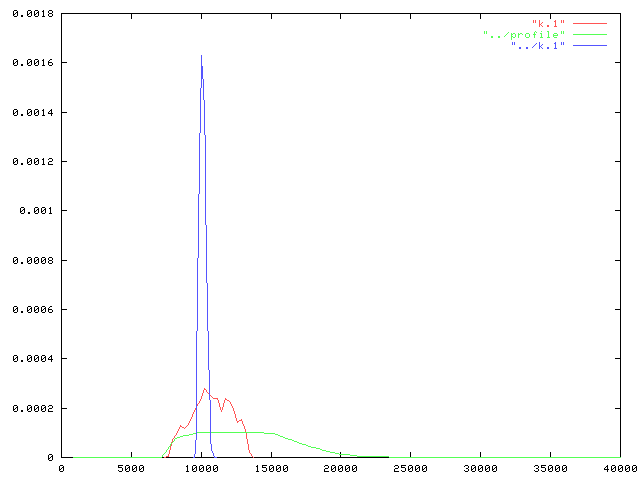
\includegraphics[height=3.5in, width=\textwidth]{mcrb3-50K.png}
\emptycaption
\label{fig:07}
\end{figure}

% !! fink.set_stepsize(.003);
% !! fink.set_stepnumber(20);

%xx \htmlnewfile

\chapter{A Forestry Model: Estimating the\br Size Distribution of
 Wildfires}
\XX{\fontindexentry{tt}{ad\_begin\_funnel}}%
{reducing the amount of temporary storage}
\X{numerical integration}

\section{Model description}

This examples highlights two features of \ADM: 1) the use of a numerical
integration routine within a statistical parameter estimation model, and 2) the
use of the \texttt{ad\_begin\_funnel} mechanism to reduce the size of temporary
file storage required. It also provides a performance comparison between \ADM\
and Splus.

This problem investigates a model that predicts a relationship between the size
and frequency of wildfires. It is assumed that the probability of observing a
wildfire in size category~$i$ is given by~$P_i$, where
\begin{equation*}
  \log(P_i)=\ln\left(S_i-S_{i+1}\right)-\ln\big(S(1)\big).
\end{equation*}
If $f_i$ is the number of widfires observed to lie in size category~$i$, the
log-likelihood function for the problem is given by
\begin{equation}
  {
l(\tau,\nu,\beta,\sigma) =
   \sum_i f_i\,\Big[\ln\big(S_i-S_{i+1}\big)-\ln\big(S(1)\big)\Big]}
\label{chp3:xx9}
\end{equation}
where $S_i$ is defined by the integral
\begin{equation}
{
  S_i=\int_{-\infty}^\infty
  \exp\Big\{-z^2/2 +
  \tau\Big(-1+\exp\big(-\nu a_i^\beta\exp(\sigma z)\big)\Big) \Big\}
  \,\textrm{d}z}
\label{chp3:xx10}
\end{equation}

The parameters $\tau$, $\nu$, $\beta$, and $\sigma$ are functions of the
parameters of the original model, and don't have a simple interpretation.
Fitting the model to data involves maximizing the above
log-likelihood~(\ref{chp3:xx9}). %xx \number\mychapno.1).
While the gradient can be calculated (in integral form), coding it is
cumbersome. Numerically maximizing the log-likelihood without specifying the
gradient is preferable.

The parameter $\beta$ is related to the fractal dimension of the perimeter of
the fire. One hypothesis of interest is that $\beta =2/3$, which is related to
hypotheses about the nature of the mechanism by which fires spread. The \ADM\
code for the model follows.
\begin{lstlisting}
DATA_SECTION
 int time0
 init_int nsteps
 init_int k
 init_vector a(1,k+1)
 init_vector freq(1,k)
 int a_index;
 number sum_freq
!! sum_freq=sum(freq);
PARAMETER_SECTION
  init_number log_tau
  init_number log_nu
  init_number log_beta(2)
  init_number log_sigma
  sdreport_number tau
  sdreport_number nu
  sdreport_number sigma
  sdreport_number beta
  vector S(1,k+1)
  objective_function_value f
INITIALIZATION_SECTION
  log_tau 0
  log_beta -.405465
  log_nu 0
  log_sigma -2
PROCEDURE_SECTION
  tau=exp(log_tau);
  nu=exp(log_nu);
  sigma=exp(log_sigma);
  beta=exp(log_beta);
   funnel_dvariable Integral;
   int i;
   for (i=1;i<=k+1;i++)
   {
     a_index=i;
     ad_begin_funnel();
     Integral=adromb(&model_parameters::h,-3.0,3.0,nsteps);
     S(i)=Integral;
   }
   f=0.0;
   for (i=1;i<=k;i++)
   {
     dvariable ff=0.0;
     // make the model stable for case when S(i)<=S(i+1)
     // we have to subrtract s(i+1) from S(i) first or roundoff will
     // do away with the 1.e-50.
     f-=freq(i)*log(1.e-50+(S(i)-S(i+1)));
     f+=ff;
   }
   f+=sum_freq*log(1.e-50+S(1));
FUNCTION dvariable h(const dvariable& z)
  dvariable tmp;
  tmp=exp(-.5*z*z + tau*(-1.+exp(-nu*pow(a(a_index),beta)*exp(sigma*z))) );
  return tmp;
REPORT_SECTION
  int * pt=NULL;
  report << " elapsed time = "  << time(pt)-time0 << " seconds" << endl;
  report << "nsteps = " << setprecision(10) <<  nsteps << endl;
  report << "f = " << setprecision(10) <<  f << endl;
  report << "a" << endl << a << endl;
  report << "freq" << endl << freq << endl;
  report << "S" << endl << S << endl;
  report << "S/S(1)" << endl << setfixed << setprecision(6) << S/S(1) << endl;
  report << "tau "  << tau << endl;
  report << "nu "  << nu << endl;
  report << "beta "  << beta << endl;
  report << "sigma "  << sigma << endl;
\end{lstlisting}

\section{The numerical integration routine}

The statement
\begin{lstlisting}
   Integral=adromb(&model_parameters::h,-3.0,3.0,nsteps);
\end{lstlisting}
invokes the numerical integration routine for the user-defined
function~\texttt{h}. The function must be defined in a \texttt{FUNCTION}
subsection. It can have any name, must be defined to take a
\texttt{const dvariable\&} argument, and must return a \texttt{dvariable}. The
values $-3.0$ and $3.0$ are the limits of integration (effectively $-\infty$,
$\infty$ for this example). The integer argument \texttt{nsteps} determines how
accurate the integration will be. Higher values of \texttt{nsteps} will be more
accurate, but greatly increase the amount of time necessary to fit the model.
The basic strategy is to use a moderate value for \texttt{nteps}, such as~6, and
then to increase this value to see if the parameter estimates change much.
\begin{lstlisting}
  FUNCTION dvariable h(const dvariable& z)
\end{lstlisting}

\section{Using the \texttt{ad\_begin\_funnel} routine to reduce\br
  the amount of temporary storage required}

Numerical integration routines can be very computationally intensive, especially
when they must be computed to great accuracy. Such computations will require a
lot of temporary storage in \ADM. Fortunately, the output from such a routine is
just one number: the value of the integral. In automatic differentiation
terminology, a long set of computations that produce just one number is known as
a ``funnel.'' It is possbile to exploit the properties of such a funnel to
greatly reduce the amount of temporary storage required. All that is necessary
is to declare an object of type \texttt{funnel\_dvariable}
\XX{\fontindexentry{tt}{funnel\_dvariable}}%
{use with\fontindexentry{tt}{ad\_begin\_funnel}}
\X{\fontindexentry{tt}{ad\_begin\_funnel}}
and to assign the results of the computation to it. At the beginning of the
funnel, a call to the function \texttt{ad\_begin\_funnel} is made. There is
quite a bit of overhead associated with the funnel construction, so it should
not be used for very small calculations. However, it is possible to put it in
and test the program to see whether or not it runs more quickly. The following
modifed code will produce exactly the same results, but without the funnel
construction:
\begin{lstlisting}
  dvariable Integral;   // change the definition of Integral
  int i;
  for (i=1;i<=k+1;i++)
  {
    a_index=i;
    // ad_begin_funnel();  // commment out this line
    Integral=adromb(&model_parameters::h,-3.0,3.0,nsteps);
    S(i)=Integral;
  }
\end{lstlisting}
If the funnel construction is used on a portion of code that is not a funnel,
incorrect derivative values will be obtained. If this is suspected, the funnel
should be removed, as in the above example, and the model run again.

\section{Effect of the accuracy switch on the\br
  running time for numerical integration}

The following report shows the amount of time required to run the model with a
fixed value of $\beta$ for different values of the parameter \texttt{nsteps}.
For practical purposes, a vlaue of \texttt{nsteps=8} gives enough accuracy so
that the model could be fit in about 6~seconds.
\begin{lstlisting}
elapsed time = 2 seconds nsteps = 6 f = 629.9846518
tau 9.851110 nu 8.913479 beta 0.666667 sigma 1.885570

elapsed time = 2 seconds nsteps = 7 f = 629.9851092
tau 9.850213 nu 8.835066 beta 0.666667 sigma 1.882967

elapsed time = 6 seconds nsteps = 8 f = 629.9851223
tau 9.850227 nu 8.836769 beta 0.666667 sigma 1.883024

elapsed time = 6 seconds nsteps = 9 f = 629.9851222
tau 9.850226 nu 8.836769 beta 0.666667 sigma 1.883024

elapsed time = 14 seconds nsteps = 10 f = 629.9851222
tau 9.850226 nu 8.836769 beta 0.666667 sigma 1.883024
\end{lstlisting}

The corresponding times when \texttt{beta} was estimated in an extra phase of
the minimization are given here. It as apparent that the model parameters become
unstable when beta is being estimated. Twice the log-likelihood difference is
$2(629.98-627.31)=5.34$ which is significant.
\begin{lstlisting}
elapsed time = 3 seconds nsteps = 6 f = 627.2919906
tau 20.729183 nu 427.816375 beta 0.180225 sigma 2.499445

elapsed time = 6 seconds nsteps = 7 f = 627.2952716
tau 21.868971 nu 80914.970724 beta 0.170392 sigma 4.232237

elapsed time = 17 seconds nsteps = 8 f = 627.297021
tau 22.858629 nu 2326271883.421848 beta 0.164749 sigma 7.653068

elapsed time = 62 seconds nsteps = 9 f = 627.2993787
tau 23.771061 nu 1652877622661391616.000000 beta 0.161073 sigma 14.451510

elapsed time = 123 seconds nsteps = 10 f = 627.3106333
tau 23.116097 nu 49753858778.636856 beta 0.159364 sigma 8.663666

elapsed time = 244 seconds nsteps = 11 f = 627.310624
tau 23.115275 nu 49009470510.133156 beta 0.159369 sigma 8.658643
\end{lstlisting}

\section{A comparison with Splus for the forestry model}

The Splus minimizing routine \texttt{nlminb} was used to fit the model. Fitting
the three-parameter model with Splus required approximately 280~seconds,
compared to 6~seconds with \ADM, so that \ADM\ was approximately 45 times faster
for this simple problem.

For the four parameter problem with beta estimated, the SPLUS routine exited
after 14~minutes and 30~seconds, reporting false convergence with a function
value of~627.338.

The data for the example is
\begin{lstlisting}
a
 0.04 0.1 0.2 0.4 0.8 1.6 3.2 6.4 12.8 25.6 51.2 102.4 204.8
freq
 167 84 61 29 19 17 4 4 1 0 1 1
\end{lstlisting}
where the first line contains the bounds for the size catagories and the second
line contains the number of observations in each size category. The Splus code
with fixed beta for the example is
\begin{lstlisting}
obj.20<-
function(xvec)
{
#Objective for maxn in NLMINB   NB vector argument
 - llik.20(xvec[1], xvec[2], xvec[3])
}
llik.20<-
function(logtau, lognu, logsigma)
{
        tau<-exp(logtau)
        nu<-exp(lognu)
        sigma<-exp(logsigma)
	print(tau)
	print(nu)
	print(sigma)
        llik <- 0
        for(i in 1:(length(freq)+1)) {
           Int[i]<-S.20(xa[i], tau, nu, sigma)
	}
        print(llik)
        for(i in 1:length(freq)) {
           llik <- llik + (freq[i] * (log(1.e-50+(Int[i]-Int[i+1]))
               -log(1.e-50+Int[1])))
        }
        llik
}
S.20<-
function(da, tau, nu, sigma)
{
        results <- integrate(intgnd.20, -3, 3, TAU = tau, NU = nu, SIGMA =
                sigma, A = da)
        if(results\$message != "normal termination")
                ans <- results\$message
        else ans <- results\$integral
        ans
}
intgnd.20<-
function(z, A, TAU, NU, SIGMA)
{
  exp(-0.5 * z^2 + TAU * (-1 + exp(-NU * A^2/3 * exp(SIGMA * z))))
}
\end{lstlisting}
To run the example in Splus with the same initial values, use the following
values
\begin{lstlisting}
  logtau 0  lognu 0  logsigma -2
\end{lstlisting}
The vector \texttt{a} should contain the 13~\texttt{a} values, while the vector
\texttt{freq} should contain the 12 observed frequencies.

%xx \htmlnewfile

\chapter{Economic Models: Regime Switching}\label{ch:regime-switching}

An active field in macroeconomic modeling is the area of ``regime switching.''
This is discussed in greater generality in \cite{hamilton1994}, Chapter~22. The
code for the following example is based on the domain switching model taken from
\cite{hamilton1989}. This example is not ideal for exploiting \ADM's greatest
advantage, which is the ability to estimate parameters in models with a large
number of independent variables. However, it does illustrate the efficacy of the
use of higher (up to 7-dimensional) arrays in \ADM.

\section{Anaylsis of economic data from \cite{hamilton1989}}

For this model, the observed quantities are the $Y_t$, where
\begin{equation}
 {
Y_t=a_0+a_1s_{ti}+Z_t}
\label{chp4:xx1}
\end{equation}
and the state variables $Z_t$ satisfy the fourth-order autoregressive
relationship
\begin{equation}
  {
Z_t=f_1Z_{t-1}+f_2Z_{t-2}+f_3Z_{t-3}+f_4Z_{t-4}+
  \epsilon_t }
\label{chp4:xx2}
\end{equation}
where, in turn, the $\epsilon_t$ are independent, normally distributed random
variables, with mean~$0$ and standard deviation~$\sigma$. These equations
correspond to Hamilton's \cite{hamilton1989} equations~4.3. The state variable
$s_{ti}$ is the realized value of a Markov process,~$S_t$, whose evolution is
described below. This coefficient takes on the value~$i$ when the system is in
state~$i$. In the current example, there are two states, so $s_t$ takes on one
of the two values~$0$ or~$1$. We can solve
equation~(\ref{chp4:xx1}) %xx $\number\mychapno.1$
for the values of $Z_t$ conditioned on the unknown value of the state at
time~$t$. Let $z_{ti}$ be defined by
\begin{align*}
  z_{i0}&=Y_t-a_0\\
  z_{t1}&=Y_t-a_0-a_1
\end{align*}

Let $(i,j,k,l,m)$ be a quintuplet of state values for the states at time
$t,t-1,\ldots,t-4$. Define~$e(t,i,j,k,l,m)$, the realized values of the random
variables~$\epsilon_t$, by
$$e(t,i,j,k,l,m)=
Y_{ti}-f_1z_{t-1,j}-f_2z_{t-2,k}
-f_3z_{t-3,l}-f_4z_{t-4,m}$$

Notice that due to the lags, we can only begin to calculate values for the
$e(t,i,j,k,l,m)$ in time period~$5$. It is assumed that the state transitions
are given by a Markov process with transition matrix
$P=(p_{ij})$.\footnote{Hamilton seems to index his matrices with the column
  index first in some cases. We use the row index first. Thus, Hamilton's
  $p_{ij}$ may correspond to our $p_{ji}$.} If we are in state~$j$ at time~$t$,
the probability of being in state~$i$ at time~$t+1$ is~$p_{ij}$.

If we consider the quintuple of the last 5 states to be the states of a new
Markov process, then we can define the transition matrix for this process by
$$(i,j,k,l,m) \Rightarrow (0,i,j,k,l)
 \hbox{\rm \quad with probability\ } p_{0i}$$
and
$$(i,j,k,l,m) \Rightarrow (1,i,j,k,l)
\hbox{\rm \quad with probability\ } p_{1i}$$ If $q(t-1,j,k,l,m,n)$ is the
probability of being in state $(j,k,l,m,n)$ at period~$t-1$, the probability of
being in state $q(t,i,j,k,l,m)$ at time period~$t$ is given by
$$q(t,i,j,l,,m)=\sum_{n}
P_{ij}q(t-1,j,k,l,m,n)$$ In particular, if $$q_b(t,i,j,k,l,m)$$ is the
probability of being in the state $(i,j,l,m,n)$ before observing $Y_t$, and
\hbox{$q_a(t-1,j,k,l,m,n)$} is the probability of being in the state
$(j,k,l,m,n)$ after observing $Y_{t-1}$, then
\begin{equation}
 {
q_b(t,i,j,k,l,m)=\sum_{n}
  P_{ij}q_a(t-1j,k,l,m,n)}
\label{chp4:xx3}
\end{equation}
Let $Q(Y_t|(i,j,k,l,m),Y_{t-1},Y_{t-2},Y_{t-3},Y_{t-4})$ be the conditional
probability (or probability density) for $Y_t$ given
$S_{t}=i,S_{t-1}=j,S_{t-2}=k,S_{t-3}=l,S_{t-4}=m,
Y_{t-1},Y_{t-2},Y_{t-3},Y_{t-4}$. Then, ignoring a constant term that is
irrelevant for the calculations,
\begin{equation}
{
Q(Y_t|(i,j,k,l,m),Y_{t-1},Y_{t-2},Y_{t-3},Y_{t-4})=
  \exp\big({}-e(i,j,k,l,m)^2/2\sigma^2\big)/\sigma }
\label{chp4:xx4}
\end{equation}
Define $u(Y_t,i,j,k,l,m)$ by
\begin{equation}
 u(Y_t,i,j,k,l,m)=
{
  Q(Y_t|(i,j,k,l,m),Y_{t-1},\ldots,Y_{t-4})
    q_b(t,i,j,k,l,m)}
\label{chp4:xx5}
\end{equation}
Then, $q_a(t,i_{t},j,k,l,m)$ can be calculated from the relationship
\begin{equation}
{
  q_a(t,i_{t},j,k,l,m)= u(Y_t,i,j,k,l,m)\kern-.2em \raisebox{-.2em}
  {\Bigg/}\kern-.7em \sum_{i,j,k,l,m} u(Y_t,i,j,k,l,m)}
\label{chp4:xx6}
\end{equation}

The log-likelihood function for the parameters can be calculated from the
$u(Y_t,i,j,k,l,m)$. It is equal to
\begin{equation}
{
\sum_t \log\raisebox{-.4em}{\Bigg(}\sum_{i,j,k,l,m}
        u(Y_t,i,j,k,l,m)\raisebox{-.4em}{\Bigg)} }
\label{chp4:xx7}
\end{equation}
% Commented out per JS 12-15-2009
% The sums needed for the calculations in
% equation~(\ref{xx}) %$\number\mychapno.9$
% can be saved from the calculations for
% equation~(\ref{xx}). % $\number\mychapno.8$).

\section{The code for Hamilton's fourth-order\br autoregressive model}

The complete \ADM\ template (\textsc{tpl}) code is in the file
\texttt{ham4.tpl}. The \cplus\ (\textsc{cpp}) code produced from this is in the
file \texttt{ham4.cpp}. Here is the \textsc{tpl} code, split up with comments:
\begin{lstlisting}
DATA_SECTION
  init_number a1init   // read in the initial value of a1 with the data
  init_int nperiods1   // the number of observations
  int nperiods  // nperiods-1 after differencing
 !! nperiods=nperiods1-1;
  init_vector yraw(1,nperiods1)  //read in the observations
  vector y(1,nperiods)   // the differenced observations
 !! y=100.*(--log(yraw(2,nperiods1)) - log(yraw(1,nperiods)));
  int order
  int op1
 !! order=4; //order of the autoregressive process
 !! op1=order+1;
  int nstates  // the number of states (expansion and contraction)
 !! nstates=2;
\end{lstlisting}
The \DS\ contains constant quantities, or ``data.'' This is in contrast to
quantities that depend on parameters being estimated, which go into the \PS. All
quantities in the \PS\ with the \texttt{init\_} prefix are initial data, which
must be read in from somewhere. By default, they are read in from the file
\texttt{ROOT.dat} (\textsc{dat} file), where ``\texttt{ROOT}'' is the root part
of the name of the program being run (in this case, \texttt{ham4.exe}, so it is
\texttt{ham4.dat}).

The first quantity is a number, \texttt{a1init}, which will be used for
initializing the value of~\texttt{a1} in the program. This is a simple way to
try different initial values for~\texttt{a1} simply by modifying the input data
file. Such procedures are often valuable, to ensure that the correct global
value of the objective function has been found. The second quantity,
\texttt{nperiods1}, is the number of data points in the file. Notice that as
soon as a quantity has been defined, it is available to use for defining other
quantities. The quantity \texttt{nperiod} does not have an \texttt{init\_}
before it, so it will not be read in and must be calulated in terms of other
quantities at some point. Since we want it now, it is calculated immediately.
\begin{lstlisting}
 !! nperiods=nperiods1-1;
\end{lstlisting}
\XX{\fontindexentry{tt}{LOCAL\_CALCS}}{\fontindexentry{tt}{!!}}
\XX{\fontindexentry{tt}{!!}}{\fontindexentry{tt}{LOCAL\_CALCS}}
The \texttt{!!} are used to insert any valid \cplus\ code into the \DS\ or
\PS. %(see \texttt{LOCAL\_CALCS}). %xx should be a \ref
This code will be executed verbatim (after the \texttt{!!} have been stripped
off, of course) at the appropriate time. The \texttt{init\_vector yraw} is
defined and given a size, with indices going from \texttt{1} to
\texttt{nperiods1}. The \texttt{nperiods1} data points will be read into
\texttt{yraw} from the \textsc{dat} file. The data are immediately transformed
and the resulting \texttt{nperiods} data points are put into~\texttt{y}.
\begin{lstlisting}
PARAMETER_SECTION
  init_vector f(1,order,1)  // coefficients for the atuoregressive
                            // process
  init_bounded_matrix Pcoff(0,nstates-1,0,nstates-1,.01,.99,2)
        // determines the transition matrix for the markov process
  init_number a0(5)  // equation 4.3 in Hamilton (1989)
  init_bounded_number a1(0.0,10.0,4);
 !! if (a0==0.0) a1=a1init;  // set initial value for a1 as specified
                     // in the top of the file nham4.dat
  init_bounded_number smult(0.01,1,3)  // used in computing sigma
  matrix z(1,nperiods,0,1)  // computed via equation 4.3 in
                          // Hamilton (1989)
  matrix qbefore(op1,nperiods,0,1);  // prob. of being in state before
  matrix qafter(op1,nperiods,0,1); // and after observing y(t)
  number sigma // variance of epsilon(t) in equation 4.3
  number var  // square of sigma
  sdreport_matrix P(0,nstates-1,0,nstates-1);
  number ff1;
  vector qb1(0,1);
  matrix qb2(0,1,0,1);
  3darray qb3(0,1,0,1,0,1);
  4darray qb4(0,1,0,1,0,1,0,1);
  6darray qb(op1,nperiods,0,1,0,1,0,1,0,1,0,1);
  6darray qa(op1,nperiods,0,1,0,1,0,1,0,1,0,1);
  6darray eps(op1,nperiods,0,1,0,1,0,1,0,1,0,1);
  6darray eps2(op1,nperiods,0,1,0,1,0,1,0,1,0,1);
  6darray prob(op1,nperiods,0,1,0,1,0,1,0,1,0,1);
  objective_function_value ff;
\end{lstlisting}
The \PS\ describes the parameters of the model, that is, the quantities to be
estimated. Quantities that have the prefix \texttt{init\_} are akin to the
independent variables from which the log-likelihood function (or, more
generally, any objective function) can be calculated. Other objects are
dependent variables that must be calculated from the independent variables. The
default behavior of \ADM\ is to read in initial parameter values for the
parameters from a \texttt{PAR} file, if it finds one. Otherwise, they are given
default values consistent with their type. The quantity~\texttt{f} is a vector
of four coefficents for the autoregressive process. \texttt{Pcoff} is a $2\times
2$ matrix used to parameterize the transition matrix \texttt{P} for the Markov
process. Its values are restricted to lie between~$0.01$ and~$0.99$.
\texttt{smult} is a number used to parameterize \texttt{sigma} and \texttt{var}
(which is the variance) as a multiple of the mean-squared residuals. This
reparameterization undimensionalizes the calculation and is a good technique to
employ for nonlinear modeling in general. The transition matrix~\texttt{P} is
defined to be of type \texttt{sdreport\_matrix}, so the standard deviation
estimates for its members will be included in the standard deviation report
contained in the \textsc{std} file. To date, \ADM\ suports up to 7-dimensional
arrays. For historical reasons, 1 and 2-dimensional arrays are referred to as
\texttt{vector} and \texttt{matrix}. This becomes a bit difficult for
higher-dimensional arrays, so they are simply referred to as \texttt{3darray},
\texttt{4darray},$\ldots$, \texttt{7darray}.
\XX{arrays}{\fontindexentry{tt}{vector}}
\XX{arrays}{\fontindexentry{tt}{matrix}}
\XX{arrays}{\fontindexentry{tt}{3darray}}
\XX{arrays}{\fontindexentry{tt}{4darray}}
\XX{arrays}{\fontindexentry{tt}{5darray}}
\XX{arrays}{\fontindexentry{tt}{6darray}}
\XX{arrays}{\fontindexentry{tt}{7darray}}
\X{\fontindexentry{tt}{3darray}}
\X{\fontindexentry{tt}{4darray}}
\X{\fontindexentry{tt}{5darray}}
\X{\fontindexentry{tt}{6darray}}
\X{\fontindexentry{tt}{7darray}}
\X{3-dimensional arrays}
\X{4-dimensional arrays}
\X{6-dimensional arrays}
\begin{lstlisting}
PROCEDURE_SECTION
  P=Pcoff;
  dvar_vector ssum=colsum(P);  // form a vector whose elements are the
                           // sums of the columns of P
  ff+=norm2(log(ssum)); // this is a penalty so that the hessian will
                        // not be singular and the coefficients of P
                        // will be well defined
  // normalize the transition matrix P so its columns sum to 1
  int j;
  for (j=0;j<=nstates-1;j++)
  {
    for (int i=0;i<=nstates-1;i++)
    {
      P(i,j)/=ssum(j);
    }
  }

  // get z into a useful format
  dvar_matrix ztrans(0,1,1,nperiods);
  ztrans(0)=y-a0;
  ztrans(1)=y-a0-a1;
  z=trans(ztrans);
  int t,i,k,l,m,n;

  qb1(0)=(1.0-P(1,1))/(2.0-P(0,0)-P(1,1)); // unconditional distribution
  qb1(1)=1.0-qb1(0);

  // for periods 2 through 4 there are no observations to condition
  // the state distributions on so we use the unconditional distributions
  // obtained by multiplying by the transition matrix P.
  for (i=0;i<=1;i++) {
    for (j=0;j<=1;j++) qb2(i,j)=P(i,j)*qb1(j);
  }

  for (i=0;i<=1;i++) {
    for (j=0;j<=1;j++) {
      for (k=0;k<=1;k++) qb3(i,j,k)=P(i,j)*qb2(j,k);
    }
  }

  for (i=0;i<=1;i++) {
    for (j=0;j<=1;j++) {
      for (k=0;k<=1;k++) {
        for (l=0;l<=1;l++) qb4(i,j,k,l)=P(i,j)*qb3(j,k,l);
      }
    }
  }

  // qb(5) is the probabilibility of being in one of 32
  // states (32=2x2x2x2x2) in periods 5,4,3,2,1 before observing
  // y(5)
  for (i=0;i<=1;i++) {
    for (j=0;j<=1;j++) {
      for (k=0;k<=1;k++) {
        for (l=0;l<=1;l++) {
          for (m=0;m<=1;m++) qb(op1,i,j,k,l,m)=P(i,j)*qb4(j,k,l,m);
        }
      }
    }
  }
  // now calculate the realized values for epsilon for all
  // possible combinations of states
  for (t=op1;t<=nperiods;t++) {
    for (i=0;i<=1;i++) {
      for (j=0;j<=1;j++) {
        for (k=0;k<=1;k++) {
          for (l=0;l<=1;l++) {
            for (m=0;m<=1;m++) {
              eps(t,i,j,k,l,m)=z(t,i)-phi(z(t-1,j),
                z(t-2,k),z(t-3,l),z(t-4,m),f);
              eps2(t,i,j,k,l,m)=square(eps(t,i,j,k,l,m));
            }
          }
        }
      }
    }
  }
  // calculate the mean squared "residuals" for use in
  // "undimensionalized" parameterization of sigma
  dvariable eps2sum=sum(eps2);
  var=smult*eps2sum/(32.0*(nperiods-4));
  sigma=sqrt(var);

  for (t=op1;t<=nperiods;t++) {
    for (i=0;i<=1;i++) {
      for (j=0;j<=1;j++) {
        for (k=0;k<=1;k++)
          prob(t,i,j,k)=exp(eps2(t,i,j,k)/(-2.*var))/sigma;
      }
    }
  }

  for (i=0;i<=1;i++) {
    for (j=0;j<=1;j++) {
      for (k=0;k<=1;k++) {
        for (l=0;l<=1;l++) {
          for (m=0;m<=1;m++) qa(op1,i,j,k,l,m)= qb(op1,i,j,k,l,m)*
            prob(op1,i,j,k,l,m);
        }
      }
    }
  }
  ff1=0.0;
  qbefore(op1,0)=sum(qb(op1,0));
  qbefore(op1,1)=sum(qb(op1,1));
  qafter(op1,0)=sum(qa(op1,0));
  qafter(op1,1)=sum(qa(op1,1));
  dvariable sumqa=sum(qafter(op1));
  qa(op1)/=sumqa;
  qafter(op1,0)/=sumqa;
  qafter(op1,1)/=sumqa;
  ff1-=log(1.e-50+sumqa);
  for (t=op1+1;t<=nperiods;t++) { // notice that the t loop includes 2
    for (i=0;i<=1;i++) {      // i,j,k,l,m blocks
      for (j=0;j<=1;j++) {
        for (k=0;k<=1;k++) {
          for (l=0;l<=1;l++) {
            for (m=0;m<=1;m++) {
              qb(t,i,j,k,l,m).initialize();
              // here is where having 6 dimensional arrays makes the
              // formula for moving the state distributions form period
              // t-1 to period t easy to program and understand.
              // Throw away  n and accumulate its two values into next
              // time period after multiplying by transition matrix P
              for (n=0;n<=1;n++) qb(t,i,j,k,l,m)+=P(i,j)*qa(t-1,j,k,l,m,n);
            }
          }
        }
      }
    }
    for (i=0;i<=1;i++) {
      for (j=0;j<=1;j++) {
        for (k=0;k<=1;k++) {
          for (l=0;l<=1;l++) {
            for (m=0;m<=1;m++) qa(t,i,j,k,l,m)=qb(t,i,j,k,l,m)*
                  prob(t,i,j,k,l,m);
          }
        }
      }
    }
    qbefore(t,0)=sum(qb(t,0));
    qbefore(t,1)=sum(qb(t,1));
    qafter(t,0)=sum(qa(t,0));
    qafter(t,1)=sum(qa(t,1));
    dvariable sumqa=sum(qafter(t));
    qa(t)/=sumqa;
    qafter(t,0)/=sumqa;
    qafter(t,1)/=sumqa;
    ff1-=log(1.e-50+sumqa); // add small constant to avoid log(0)
  }
  ff+=ff1; //ff1 is minus the log-likelihood
  ff+=.1*norm2(f); // add small penalty to stabilize estimation
\end{lstlisting}
The \PROS\ is where the calculations of the objective function are carried out.
First, the transition matrix \texttt{P} is calculated from the \texttt{Pcoff}.
The function \texttt{colsum} forms a vector whose elements are the column sums
of the matrix. This is used to normalize \texttt{P} so that its columns sum
to~$1$. A penalty is added to the objective function for the column sums, so the
Hessian matrix with respect to the independent variables will not be singular.
This does not affect the ``statistical'' properties of the parameters of
interest. The matrix~\texttt{z} is calculated using a transformed matrix,
because \ADM\ deals with vector rows better than columns. The probability
distribution for the states in period~1, \texttt{qb1}, is set equal to the
uncondtional distribution for a Markov process in terms of its transition matrix
\texttt{P}, as discussed in~\cite{hamilton1994}. The transition matrix is used
to compute the probability distribution of the states in periods $(2,1)$,
$(3,2,1)$, $(4,3,2,1)$, and finally, $(5,4,3,2,1)$. For the last quintuplet,
this is the probability distribution before observing~\texttt{y(5)}. The
quantities \texttt{eps} in the code correspond to the possible realized values
of the random variable~$\epsilon$. The quantities \texttt{qa} and \texttt{qb}
correspond to $q_a$ and $q_b$ in the documentation. The \texttt{sum} function is
defined for arrays of any dimension and simply forms the sum of all the
components. In \ADM, if \texttt{xx} is an $n$-dimensional array, then
\texttt{x(i)} is an $(n-1)$-dimensional array. So, the statement
\begin{lstlisting}
    qbefore(t,0)=sum(qb(t,0));
\end{lstlisting}
takes the sum of the probabilities for the 16 quintuples of states, at time
period~\texttt{t} through~\texttt{t-4}, for which the state at time
period~\texttt{t} is~$0$. These are used in the \RS, to write out a report of
the estimated state probabilities at time period \texttt{t}, before and after
observing~\texttt{y(t)}.
\begin{lstlisting}
REPORT_SECTION
  dvar_matrix out(1,2,op1,nperiods);
  dvar_matrix out1(1,1,op1,nperiods);
  out(1)=trans(qbefore)(1);
  out(2)=trans(qafter)(1);
  {
    ofstream ofs("qbefore.rep");
    out1(1)=trans(qbefore)(0);
    ofs << trans(out1)<< endl;
  }
  {
    ofstream ofs("qafter.rep");
    out1(1)=trans(qafter)(0);
    ofs << trans(out1) << endl;
  }
  report << "#qbefore    qafter" <<  endl;
  report << setfixed << setprecision(3) << setw(7) << trans(out) << endl;
\end{lstlisting}
\XX{\fontindexentry{tt}{REPORT\_SECTION}}{example of}
The \RS\ is used to report any result in a manner not already carried out by the
model's default behavior. The probabilites of being in state~$0$ before and
after observing \texttt{y(t)} are printed into the files \texttt{qbefore.rep}
and \texttt{qafter.rep}. These vectors were stored in files, so they could be
easily imported into graphing programs. The results are very similar to Figure~1
in~\cite{hamilton1989}, as one might hope.
\begin{lstlisting}
RUNTIME_SECTION
  maximum_function_evaluations 20000
  convergence_criteria 1.e-6
\end{lstlisting}
\X{\fontindexentry{tt}{convergence\_criteria}}
\X{\fontindexentry{tt}{maximum\_function\_evaluations}}
The \texttt{maximum\_function\_evaluations 20000} will simply let the program
run a long time by setting the maximum number of function evaluations in the
function minimizer equal to 20,000. (Nowhere near this many are actually
needed.) The statement
\begin{lstlisting}
  convergence_criteria 1.e-6
\end{lstlisting}
was needed, because the default value of \texttt{1.e-4} caused the program to
exit from the miniization before convergence had been achieved.
\X{\fontindexentry{tt}{arrmblsize}}
\X{\fontindexentry{tt}{TOP\_OF\_MAIN} section}
\XX{\fontindexentry{tt}{gradient\_structure::}}%
{\fontindexentry{tt}{set\_ARRAY\_MEMBLOCK\_SIZE, the correct way to set}}
\XX{\fontindexentry{tt}{gradient\_structure::}}%
{\fontindexentry{tt}{set\_GRADSTACK\_BUFFER\_SIZE}}
\begin{lstlisting}
TOP_OF_MAIN_SECTION
  arrmblsize=500000;
  gradient_structure::set_GRADSTACK_BUFFER_SIZE(200000);
  gradient_structure::set_CMPDIF_BUFFER_SIZE(2100000);
\end{lstlisting}
The \texttt{TOP\_OF\_MAIN\_SECTION} is for including code that will be included
at the top of the \texttt{main()} function in the \cplus\ program. Any desired
legal code may be included. There are a number of common statements that are
used to control aspects of \ADM's performance. The statement
\begin{lstlisting}
  arrmblsize=500000;
\end{lstlisting}
reserves 500,000 bytes of memory for variable objects. If it is not large
enough, a message will be printed out at run time. See the index for references
to more discussions of this matter. The statements
\begin{lstlisting}
  gradient_structure::set_GRADSTACK_BUFFER_SIZE(200000);
\end{lstlisting}
and
\begin{lstlisting}
  gradient_structure::set_CMPDIF_BUFFER_SIZE(2100000);
\end{lstlisting}
set the amount of memory that \ADM\ reserves for variable objects. Setting these
is a matter of tuning for optimum performance. If you have a lot of memory
available, making them larger may improve performance. However, models will run
without including these statements, as long as there is enough memory for \ADM's
temporary files.
\X{\fontindexentry{tt}{ GLOBALS\_SECTION}}
\begin{lstlisting}
GLOBALS_SECTION
  #include <admodel.h>

  dvariable phi(const dvariable& a1,const dvariable& a2,const dvariable& a3,
    const dvariable& a4,const dvar_vector& f)
  {
    return   a1*f(1)+a2*f(2)+a3*f(3)+a4*f(4);
  }
\end{lstlisting}
The \texttt{GLOBALS\_SECTION} is used to include statements at the top of the
file containing the \textsc{cpp} program. This is generally where global
declarations are made in \cplus, hence its name. However, it may be used for any
legal statments, such as including header files for the user's data structures,
etc. In this case, it has been used to define the function~\texttt{phi}, which
is used to simplify the code for the model's calculations. The header file
\texttt{admodel.hpp} is included, to define the \scAD\ structures used in the
definition of the function. This header is automatically included near the top
of the file, but this would be too late, as \texttt{GLOBALS\_SECTION} material
is included first.

\section{Results of the analysis}

The parameter estimates for the initial parameters are written into a file
\texttt{HAM4.PAR}. This is an \textsc{ascii} file, which can be easily read.
(The results are also stored in a binary file \texttt{HAM4.BAR}, which can be
used to restart the model with more accurate parameters estimates.)
\begin{lstlisting}
# Objective function value = 60.8934
# f:
 0.0139989 -0.0569580 -0.246292 -0.212250
# Pcoff:
 0.754133 0.0955834
 0.245118 0.900333
# a0:
-0.357964
# a1:
1.52138
# smult:
0.281342
\end{lstlisting}
The estimates are almost identical to those reported in
\cite{hamilton1989}\footnote{Our method for parameterizing the intial state
  probability distribution \texttt{qb1} is slightly different from Hamilton's,
  which would explain the small discrepancy.} The first line reports the value
of the log-likelihood function. This value can be used in hypothesis
(likelihood-ratio) tests. The file \texttt{ham5.para} for the fifth-order
autoregressive model fit to the data in \cite{hamilton1989} is shown below.
There is one more parameter in this model. Twice the difference in the
log-likelihood functions is $2(60.89-59.60)=2.58$. For one extra parameter, the
$95\%$ significance level is $3.84$, so the improvement in fit is not
significant.

\begin{lstlisting}
# Objective function value = 59.6039
# f:
 -0.0474771 -0.113829 -0.241966 -0.225535 -0.192585
# Pcoff:
 0.779245 0.0951739
 0.219775 0.900719
# a0:
-0.271318
# a1:
1.46301
# smult:
0.259541
\end{lstlisting}

The plot of \texttt{qa} and \texttt{qb} demonstrates the extra information about
the probability distribution of the current state contained in in the current
value of~\texttt{y(t)}. (See Figure~\ref{fig:08}.)
\begin{figure}[h]
\centering\hskip1pt\beginpicture
  \setplotsymbol ({\eightrm .})
  \setcoordinatesystem units <3.2in,2.5in>
  \setplotarea x from -0.02 to 1.3, y from -.02 to 1.02
  \axis left
  /
  \axis left
    ticks numbered from .0 to 1.0 by .2
  /
\linethickness .8 truept
\setdashpattern <1pt,1pt,1pt,1pt>
{
   \color{red}
   %\setcolor\cmykRed  % turn on color
   %%  \setcolor\cmykSeaGreen  % turn on color
 \plot  "qbefore4.tex"
   \color{blue}
   %\setcolor\cmykMidnightBlue  % turn on color
\setdashpattern <1pt,3pt,4pt,3pt>
 \plot  "qafter4.tex"
   \color{red}
   %\setcolor\cmykRed  % turn on color
 \put {\hbox{\texttt{ qb }}} at .43 0.9
 \putrule from .48 .9 to .64 0.9
   \color{blue}
   %\setcolor\cmykMidnightBlue  % turn on color
 \put {\mbox{\texttt{ qa }}} at .43 .8
 \putrule from .48 .8 to .64 .8
   \color{black}
   %\setcolor\cmykBlack  % turn on color
}
% \put {\hbox\texttt{qb }} at .43 0.9
% \putrule from .48 .9 to .64 0.9
%\setdashpattern <1pt,3pt,4pt,3pt>
%{
  % \setcolor\cmykMidnightBlue  % turn on color
 %\plot  "qafter4.tex"
%}
 %\put {\hbox\texttt{qa }} at .43 .8
% \putrule from .48 .8 to .64 .8
\endpicture
% \vbox{
% \hbox{
% \beginpicture
%   \setplotsymbol ({\eightrm .})
%   \setcoordinatesystem units <3.2in,2.0in>
%   \setplotarea x from -0.02 to 1.3, y from -.02 to 1.02
%   \axis left
%   /
%   \axis bottom label {Aposteriori
%      Probabilitites of Being in State 0 in Period t}
%   /
%   \axis left
%     ticks
%     numbered from .0 to 1.0 by .2
%   /
% \linethickness .8 truept
% \setdashpattern <1pt,1pt,1pt,1pt>
% % \plot  "qbefore4.tex"
%  \put {\hbox\texttt{qb }} at .43 0.9
%  \putrule from .48 .9 to .64 0.9
% \setdashpattern <1pt,3pt,4pt,3pt>
%  \plot  "qafter4.tex"
%  \put {\hbox\texttt{qa }} at .43 .8
%  \putrule from .48 .8 to .64 .8
% \endpicture
% \hfill
% }}
\bigskip
\medskip
\par
\raggedright
The standard deviation and correlation report for the model are in the file
\texttt{ham4.cor}, reproduced below:\par
\centering
%xx \htmlbegintex
\begin{smallcode}[commentchar=\%]
 index name  value    std.dev    1     2     3     4     5     6     7     8%
     9    10    11    12    13    14   15
   1  f      1.39e-02 1.20e-01  1.00
   2  f     -5.69e-02 1.37e-01  0.33  1.00
   3  f     -2.46e-01 1.06e-01  0.33  0.29  1.00
   4  f     -2.12e-01 1.10e-01  0.43  0.26  0.17  1.00
   5  Pcoff  7.54e-01 5.39e-01  0.00  0.04  0.01  0.00  1.00
   6  Pcoff  9.55e-02 7.58e-02  0.04  0.05  0.02  0.03 -0.04  1.00
   7  Pcoff  2.45e-01 1.97e-01 -0.01 -0.11 -0.03 -0.01  0.77  0.04  1.00
   8  Pcoff  9.00e-01 6.20e-01 -0.00 -0.00 -0.00 -0.00  0.00  0.83 -0.00  1.00
   9  a0    -3.57e-01 2.65e-01  0.27  0.56  0.25  0.21  0.08  0.07 -0.23 -0.00%
  1.00
  10  a1     1.52e+00 2.63e-01 -0.31 -0.57 -0.29 -0.25 -0.07 -0.04  0.21  0.00%
 -0.96  1.00
  11  smult  2.81e-01 1.25e-01  0.54  0.69  0.48  0.45  0.06  0.05 -0.17 -0.00%
  0.82 -0.84  1.00
  12  P      7.54e-01 9.65e-02  0.02  0.24  0.07  0.03  0.17 -0.08 -0.48  0.00%
  0.47 -0.44  0.36  1.00
  13  P      9.59e-02 3.77e-02  0.09  0.10  0.04  0.06 -0.02  0.49  0.08 -0.05%
  0.14 -0.09  0.11 -0.16  1.00
  14  P      2.45e-01 9.65e-02 -0.02 -0.24 -0.07 -0.03 -0.17  0.08  0.48 -0.00%
 -0.47  0.44 -0.36 -1.00  0.16  1.00
  15  P      9.04e-01 3.77e-02 -0.09 -0.10 -0.04 -0.06  0.02 -0.49 -0.08  0.05%
 -0.14  0.09 -0.11  0.16 -1.00 -0.16 1.00
\end{smallcode}
\caption{Apriori and aposteriori probabilitites of being in state 0 in period
  $t$.}
\label{fig:08}
\end{figure}
%xx \htmlendtex

\section{Extending Hamilton's model to a\br fifth-order autoregressive process}

Hamilton \cite{hamilton1989}, page~372, remarks that investigating higher-order
autoregressive processes might be a fruitful area of research.
%The form of the model is. %xx is there something missing here?
The first extension of the model is a fifth-order autoregressive process.
\begin{equation}
{
Y_t=a_0+a_1s_{ti}+Z_t }
\label{chp5:yy1}
\end{equation}
and the state variables $Z_t$ satisfy the fourth-order autoregressive
relationship
\begin{equation}
{
Z_t=f_1Z_{t-1}+f_2Z_{t-2}+f_3Z_{t-3}+f_4Z_{t-4}+f_5Z_{t-5}+
  \epsilon_t}
\label{chp5:yy2}
\end{equation}
which extend equations (\ref{chp4:xx1}) %xx \number\mychapno.1
and (\ref{chp4:xx2}). %xx \number\mychapno.2.
The \textsc{tpl} file \texttt{ham5.tpl} for the fifth-order autoregressive model
is reproduced here. By employing higher-dimensional arrays, the conversion of
the \textsc{tpl} file from a fourth-order autoregressive process to a
fifth-order one is largely formal. An experienced \ADM\ user can carry out the
modifications in under one hour. Places where modifications were made are tagged
with the comment~\texttt{//!!5}.
\begin{lstlisting}
DATA_SECTION
  init_number a1init   // read in the initial value of a1 with the data
  init_int nperiods1   // the number of observations
  int nperiods  // nperiods-1 after differencing
 !! nperiods=nperiods1-1;
  init_vector yraw(1,nperiods1)  //read in the observations
  vector y(1,nperiods)   // the differenced observations
 !! y=100.*(--log(yraw(2,nperiods1)) - log(yraw(1,nperiods)));
  int order
  int op1
 !! order=5; // !!5 order of the autoregressive process
 !! op1=order+1;
  int nstates  // the number of states (expansion and contraction)
 !! nstates=2;
PARAMETER_SECTION
  init_vector f(1,order,1)  // coefficients for the atuoregressive
                            // process
  init_bounded_matrix Pcoff(0,nstates-1,0,nstates-1,.01,.99,2)
        // determines the transition matrix for the markov process
  init_number a0(5)  // equation 4.3 in Hamilton (1989)
  init_bounded_number a1(0.0,10.0,4);
 !! if (a0==0.0) a1=a1init;  // set initial value for a1 as specified
                     // in the top of the file nham4.dat
  init_bounded_number smult(0.01,1,3)  // used in computing sigma
  matrix z(1,nperiods,0,1)  // computed via equation 4.3 in
                          // Hamilton (1989)
  matrix qbefore(op1,nperiods,0,1);  // prob. of being in state before
  matrix qafter(op1,nperiods,0,1); // and after observing y(t)
  number sigma // variance of epsilon(t) in equation 4.3
  number var  // square of sigma
  sdreport_matrix P(0,nstates-1,0,nstates-1);
  number ff1;
  vector qb1(0,1);
  matrix qb2(0,1,0,1);
  3darray qb3(0,1,0,1,0,1);
  4darray qb4(0,1,0,1,0,1,0,1);
  5darray qb5(0,1,0,1,0,1,0,1,0,1); // !!5
  7darray qb(op1,nperiods,0,1,0,1,0,1,0,1,0,1,0,1);
  7darray qa(op1,nperiods,0,1,0,1,0,1,0,1,0,1,0,1);
  7darray eps(op1,nperiods,0,1,0,1,0,1,0,1,0,1,0,1);
  7darray eps2(op1,nperiods,0,1,0,1,0,1,0,1,0,1,0,1);
  7darray prob(op1,nperiods,0,1,0,1,0,1,0,1,0,1,0,1);
  objective_function_value ff;
PROCEDURE_SECTION
  P=Pcoff;
  dvar_vector ssum=colsum(P);  // form a vector whose elements are the
                           // sums of the columns of P
  ff+=norm2(log(ssum)); // this is a penalty so that the Hessian will
                        // not be singular and the coefficients of P
                        // will be well defined
  // normalize the transition matrix P so its columns sum to 1
  int j;
  for (j=0;j<=nstates-1;j++)
  {
    for (int i=0;i<=nstates-1;i++)
    {
      P(i,j)/=ssum(j);
    }
  }

  dvar_matrix ztrans(0,1,1,nperiods);
  ztrans(0)=y-a0;
  ztrans(1)=y-a0-a1;
  z=trans(ztrans);
  int t,i,k,l,m,n,p;

  qb1(0)=(1.0-P(1,1))/(2.0-P(0,0)-P(1,1)); // unconditional distribution
  qb1(1)=1.0-qb1(0);

  // for periods 2 through 4 there are no observations to condition
  // the state distributions on so we use the unconditional distributions
  // obtained by multiplying by the transition matrix P.
  for (i=0;i<=1;i++) {
    for (j=0;j<=1;j++) qb2(i,j)=P(i,j)*qb1(j);
  }

  for (i=0;i<=1;i++) {
    for (j=0;j<=1;j++) {
      for (k=0;k<=1;k++) qb3(i,j,k)=P(i,j)*qb2(j,k);
    }
  }

  for (i=0;i<=1;i++) {
    for (j=0;j<=1;j++) {
      for (k=0;k<=1;k++) {
        for (l=0;l<=1;l++) qb4(i,j,k,l)=P(i,j)*qb3(j,k,l);
      }
    }
  }
  // !!5
  for (i=0;i<=1;i++) {
    for (j=0;j<=1;j++) {
      for (k=0;k<=1;k++) {
        for (l=0;l<=1;l++) {
          for (m=0;m<=1;m++) qb5(i,j,k,l,m)=P(i,j)*qb4(j,k,l,m);
	}
      }
    }
  }
  // qb(6) is the probabilibility of being in one of 64
  // states (64=2x2x2x2x2x2) in periods 5,4,3,2,1 before observing
  // y(6)
  for (i=0;i<=1;i++) {
    for (j=0;j<=1;j++) {
      for (k=0;k<=1;k++) {
        for (l=0;l<=1;l++) {
          for (m=0;m<=1;m++) { // !!5
            for (n=0;n<=1;n++) qb(op1,i,j,k,l,m,n)=P(i,j)*qb5(j,k,l,m,n);
          }
	}
      }
    }
  }
  // now calculate the realized values for epsilon for all
  // possible combinations of states
  for (t=op1;t<=nperiods;t++) {
    for (i=0;i<=1;i++) {
      for (j=0;j<=1;j++) {
        for (k=0;k<=1;k++) {
          for (l=0;l<=1;l++) {
            for (m=0;m<=1;m++) {
              for (n=0;n<=1;n++) { // !!5
	        eps(t,i,j,k,l,m,n)=z(t,i)-phi(z(t-1,j),
	          z(t-2,k),z(t-3,l),z(t-4,m),z(t-5,n),f);
                eps2(t,i,j,k,l,m,n)=square(eps(t,i,j,k,l,m,n));
              }
	    }
	  }
	}
      }
    }
  }
  // calculate the mean squared "residuals" for use in
  // "undimensionalized" parameterization of sigma
  dvariable eps2sum=sum(eps2);
  var=smult*eps2sum/(64.0*(nperiods-4));  //!!5
  sigma=sqrt(var);

  for (t=op1;t<=nperiods;t++) {
    for (i=0;i<=1;i++) {
      for (j=0;j<=1;j++) {
        for (k=0;k<=1;k++) {
          for (l=0;l<=1;l++)  //!!5
	    prob(t,i,j,k,l)=exp(eps2(t,i,j,k,l)/(-2.*var))/sigma;
        }
      }
    }
  }

  for (i=0;i<=1;i++) {
    for (j=0;j<=1;j++) {
      for (k=0;k<=1;k++) {
        for (l=0;l<=1;l++) {
          for (m=0;m<=1;m++) {
            for (n=0;n<=1;n++) qa(op1,i,j,k,l,m,n)= qb(op1,i,j,k,l,m,n)*
	      prob(op1,i,j,k,l,m,n);
          }
        }
      }
    }
  }
  ff1=0.0;
  qbefore(op1,0)=sum(qb(op1,0));
  qbefore(op1,1)=sum(qb(op1,1));
  qafter(op1,0)=sum(qa(op1,0));
  qafter(op1,1)=sum(qa(op1,1));
  dvariable sumqa=sum(qafter(op1));
  qa(op1)/=sumqa;
  qafter(op1,0)/=sumqa;
  qafter(op1,1)/=sumqa;
  ff1-=log(1.e-50+sumqa);
  for (t=op1+1;t<=nperiods;t++) { // notice that the t loop includes 2
    for (i=0;i<=1;i++) {      // i,j,k,l,m blocks
      for (j=0;j<=1;j++) {
        for (k=0;k<=1;k++) {
          for (l=0;l<=1;l++) {
            for (m=0;m<=1;m++) {
              for (n=0;n<=1;n++) { //!!5
                qb(t,i,j,k,l,m,n).initialize();
	        // here is where having 6 dimensional arrays makes the
	        // formula for moving the state distributions form period
	        // t-1 to period t easy to program and understand.
	        // Throw away  n and accumulate its two values into next
	        // time period after multiplying by transition matrix P
                for (p=0;p<=1;p++) qb(t,i,j,k,l,m,n)+=P(i,j)*
		  qa(t-1,j,k,l,m,n,p);
              }
            }
	  }
	}
      }
    }
    for (i=0;i<=1;i++) {
      for (j=0;j<=1;j++) {
        for (k=0;k<=1;k++) {
          for (l=0;l<=1;l++) {
            for (m=0;m<=1;m++) { // !!5
              for (n=0;n<=1;n++) qa(t,i,j,k,l,m,n)=qb(t,i,j,k,l,m,n)*
	          prob(t,i,j,k,l,m,n);
            }
	  }
	}
      }
    }
    qbefore(t,0)=sum(qb(t,0));
    qbefore(t,1)=sum(qb(t,1));
    qafter(t,0)=sum(qa(t,0));
    qafter(t,1)=sum(qa(t,1));
    dvariable sumqa=sum(qafter(t));
    qa(t)/=sumqa;
    qafter(t,0)/=sumqa;
    qafter(t,1)/=sumqa;
    ff1-=log(1.e-50+sumqa);
  }
  ff+=ff1;
  ff+=.1*norm2(f);
REPORT_SECTION
  dvar_matrix out(1,2,op1,nperiods);
  out(1)=trans(qbefore)(1);
  out(2)=trans(qafter)(1);
  {
    ofstream ofs("qbefore4.tex");
    for (int t=5;t<=nperiods;t++)
    {
      ofs << (t-4)/100. << " " << qbefore(t,0) << endl;
    }
  }
  {
    ofstream ofs("qafter4.tex");
    for (int t=5;t<=nperiods;t++)
    {
      ofs << (t-4)/100. << " " << qafter(t,0) << endl;
    }
  }
  report << "#qbefore    qafter" <<  endl;
  report << setfixed << setprecision(3) << setw(7) << trans(out) << endl;
RUNTIME_SECTION
  maximum_function_evaluations 20000
  convergence_criteria 1.e-6
TOP_OF_MAIN_SECTION
  arrmblsize=500000;
  gradient_structure::set_GRADSTACK_BUFFER_SIZE(400000);
  gradient_structure::set_CMPDIF_BUFFER_SIZE(2100000);
  gradient_structure::set_MAX_NVAR_OFFSET(500);
GLOBALS_SECTION
  #include <fvar.hpp>
   // !!5
  dvariable phi(const dvariable& a1,const dvariable& a2,const dvariable& a3,
    const dvariable& a4,const dvariable& a5,const dvar_vector& f)
  {
    return   a1*f(1)+a2*f(2)+a3*f(3)+a4*f(4)+a5*f(5);
  }
\end{lstlisting}

%xx \htmlnewfile
\chapter{Econometric Models:\br Simultaneous Equations}
\input simequat.tex%xxread \x

%xx \htmlnewfile
\chapter{Truncated Regression}
\input truncreg.tex %xxread \x

%xx \htmlnewfile
\chapter{Multivariate \textsc{garch}}
\input magarch-april2000.tex %xxread \x

%xx \htmlnewfile
\chapter{The Kalman Filter}
\input kalman.tex%xxread \x

%xx \htmlnewfile
\chapter{Applying the Laplace Approximation\br
  to the Generalized Kalman Filter:\br
  with an Application to Stochastic Volatility Models}
\input kal_lap.tex%xxread \x

%xx \htmlnewfile
\chapter{Using Vectors of Initial Parameter Types}
\input advectors.tex%xxread \x

%xx \htmlnewfile
\chapter{Creating Dynamic Link Libraries\br with \ADM}
\input admb-dll.tex %xxread \x

%xx \htmlnewfile
\chapter{Command Line Options}
\input commandl.tex%xxread \x

%xx \htmlnewfile
%\chapter{Parallel Processing on Clusters}
%\input parallel1.tex
%\endchapter

%xx \htmlnewfile
\chapter{Writing Adjoint Code}
\input adjoint.tex%xxread \x

%%xx \htmlnewfile
%\chapter{The Random Effects Module}
%\input randeff.tex
%\endchapter

% %xx \htmlnewfile
% \chapter{Nonlinear state space models---beyond the Kalman Filter---the
% Holistic approach}
% \input nlss2
% \endchapter

%xx \htmlnewfile
\chapter{Truncated Regression}
\input truncreg.tex%xxread \x

%xx \htmlnewfile
\chapter{All the Functions in \ADM}
\input allfun.tex %xxread \x

%xx \htmlnewfile
\chapter{Miscellaneous and Advanced Features\br of \ADM}
\X{\fontindexentry{tt}{adstring} class}
\XX{strings}{reading from \fontindexentry{sc}{dat} file}

\section{Using strings and labels in the \textsc{tpl} file}

For purposes of this manual, a ``label'' is a string that does not have any
blanks in it. Such strings can be read in from the \texttt{data} file using the
\texttt{init\_adstring} declaration, as in
\begin{lstlisting}
DATA_SECTION
  init_adstring s
\end{lstlisting}
The \textsc{dat} file should contain something like
\begin{lstlisting}
# label to be read in
  my_model_data
\end{lstlisting}
When the program runs, the \texttt{adstring} object \texttt{s} should contain
the string
\begin{lstlisting}
  my_model_data
\end{lstlisting}
White space at the beginning is ignored and following white space terminates the
input of the object.

Discussions of the various operations on \texttt{adstring} class members are
found elsewhere in the manual.

\section{Using other class libraries in\br \ADM\ programs}

\XX{Using other \cplus\ classes in \ADM}{\fontindexentry{tt}{!!CLASS}}
A useful feature of \cplus\ is its open nature. This means that the user can
combine several class libraries into one program. In general, this simply
involves including the necessary header files in the program and then declaring
the appropriate class instances in the program. Instances of external classes
can be declared in an \ADM\ program in several ways. They can always be declared
in the procedure or report section of the program as local objects. It is
sometimes desired to include instances of external classes in a more formal way
into an \ADM\ program. This section describes how to include them into the \DS\
or \PS. After that, they can be referred to as though they were part of the
\ADM\ code (except for the technicalities to be discussed below).

\ADM\ employs a strategy of late initialization of class members. The reason for
this is to allow time for the user to carry out any calculations that may be
necessary for determining parameter values, etc., that are used in the
initialization of the object. Because of the nature of constructors in \cplus,
this means that every object declared in the \DS\ or the \PS\ must have a
default constructor that takes no arguments. The actual allocation of the object
is carried out by a class member function named \texttt{allocate}, which takes
any desired arguments. Since external classes will not generally satisfy these
requirements, a different strategy is employed for these classes. A pointer to
the object is included in the appropriate \ADM\ class. This pointer has the
prefix \texttt{pad\_} inserted before the name of the object. The pointer to
\texttt{myobj} would have the form \texttt{pad\_myobj}.
\begin{lstlisting}
 !!CLASSfooclass myobj( ...)
\end{lstlisting}
The user can refer to the object in the code simply by using its name.

\appendix

\chapter{The Regression Function}\label{ch:appendix-regression-function}

The \texttt{robust\_regression} function calculates the log-likelihood function
for the standard statistical model of independent normally distributed errors,
with mean~0 and equal variance. The code is written in terms of \scAD\ objects,
such as \texttt{dvariable} and \texttt{dvar\_vector}. They are described in the
\scAD\ user's manual.
\begin{lstlisting}
dvariable regression(const dvector& obs,const dvar_vector& pred)
{
  double nobs=double(size_count(obs));  // get the number of
                                        // observations
  dvariable vhat=norm2(obs-pred);  // sum of squared deviations
  vhat/=nobs;                      //mean of squared deviations
  return (.5*nobs*log(vhat));     //return log-likelihood value
}
\end{lstlisting}

\chapter{\ADM\ Types}

The effect of a declaration depends on whether or not it occurs in the \DS\ or
in the \PS. Objects declared in the \DS\ are constant, that is, like data.
Objects declared in the \PS\ are variable, that is, like the parameters of the
model that are to be estimated. Any objects that depend on variable objects must
themselves be variables objects, that is, they are declared in the \PS\ and not
in the \DS.

In the \DS, the prefix \texttt{init\_} indicates that the object is to be read
in from the data file. In the \PS, the prefix indicates that the object is an
initial parameter whose value will be used to calculate the value of other
(non-initial) parameters. In the \PS, initial parameters will either have their
values read in from a parameter file or will be initialized with their default
initial values. The actual default values used can be modified in the
\texttt{INITIALIZATION\_SECTION}. From a mathematical point of view, objects
declared with the \texttt{init\_} prefix are independent variables that are used
to calculate the objective function being minimized.
\X{\fontindexentry{tt}{INITIALIZATION\_SECTION}}
\X{3-dimensional arrays}

The prefixes \texttt{bounded\_} and \texttt{dev\_} can only be used in the \PS.
The prefix \texttt{bounded\_} restricts the numerical values that an object can
take on to lie in a specified bounded interval. The prefix \texttt{dev\_} can
only be applied to the declaration of vector objects. It has the effect of
restricting the individual components of the vector object so that they sum to
zero.

The prefix \texttt{sdreport\_} can only be used in the \PS. An object declared
with this prefix will appear in the covariance matrix report. This provides a
convenient method for obtaining estimates for the variance of any parameter that
may be of interest. Note that the prefixes \texttt{sdreport\_} and
\texttt{init\_} cannot both be applied to the same object. There is no need to
do so, since initial parameters are automatically included in the standard
deviations report. \ADM\ also has 3 and 4-dimensional arrays. They are
declared~like
\XX{arrays}{3-dimensional}
\XX{arrays}{3-dimensional}
\X{3-dimensional arrays}
\X{4-dimensional arrays}
\begin{lstlisting}
3darray dthree(1,10,2,20,3,10)
4darray df(1,10,2,20,3,10)
init_3darray dd(1,10,2,20,3,10)    // data section only
init_4darray dxx(1,10,2,20,3,10)   // data section only
\end{lstlisting}
Table~\ref{tab:type-declarations} contains a summary of declarations and the
types of objects associated with them in \ADM. The types
\texttt{dvariable, dvector, dmatrix, d3\_array, dvar\_vector, dvar\_matrix}, and
\texttt{dvar3\_array} are described in the \scAD\ users's manual.

%xx \htmlbegintex

\begin{table}
\bgroup\footnotesize
\noindent\begin{tabular}{@{\vrule height 12pt depth 6pt width0pt}%
    @{\tt} l @{\qquad} l @{\qquad}  l}
\\
\hline
{\bf Declaration} & {\bf Type of object} & {\bf Type of object} \\[2pt]
\hline
&in \DS & in \PS \\[1em]
{[}init\_]int & int & int \\
{[}init\_]{[}bounded\_]number & double & \texttt{dvariable} \\
{[}init\_]{[}bounded\_]{[}dev\_]vector & vector of doubles (\texttt{dvector})
& vector of \texttt{dvariables(dvar\_vector)} \\
{[}init\_]{[}bounded\_]matrix & matrix of doubles (\texttt{dmatrix})
& matrix of \texttt{dvariables(dvar\_matrix)} \\
{[}init\_]3darray & 3-dimensional array of doubles
& 3-dimensional array of \texttt{dvariables} \\
4darray & 4-dimensional array of doubles
& 4-dimensional array of \texttt{dvariables} \\
5darray & 5-dimensional array of doubles
& 5-dimensional array of \texttt{dvariables} \\
6darray & 6-dimensional array of doubles
& 6-dimensional array of \texttt{dvariables} \\
7darray & 7-dimensional array of doubles
& 7-dimensional array of \texttt{dvariables} \\
sdreport\_number & N/A &\texttt{dvariable} \\
likeprof\_number & N/A &\texttt{dvariable} \\
sdreport\_vector & N/A &vector of \texttt{dvariables(dvar\_vector)} \\
sdreport\_matrix & N/A &matrix of \texttt{dvariables(dvar\_matrix)} \\[3pt]
\hline
\\
\end{tabular}
\emptycaption
\label{tab:type-declarations}
\egroup
\end{table}
%xx \htmlendtex

\chapter{The Profile Likelihood}
\X{profile likelihood}
\XX{profile likelihood}{form of calculations}

We have been told that the profile likelihood as calculated in \ADM\ for
dependent variables may differ from that calculated by other authors. This
section will clarify what we mean by the term and motivate our calculation.

Let $(x_1,\ldots,x_n)$ be $n$ independent variables, $f(x_1,\ldots,x_n)$ be a
probability distribution, and $g$ denote a dependent variable that is a real
valued function of $(x_1,\ldots,x_n)$. Fix a value~$g_0$ for $g$ and consider
the integral
$$\int_{\{x:g_0-\epsilon/2\le g(x)\le g_0+\epsilon/2\}} f(x_1,\ldots, x_n)$$
which is the probability that $g(x)$ has a value between $g_0-\epsilon/2$ and
$g_0+\epsilon/2$. This probability depends on two quantities: the value of
$f(x)$ and the thickness of the region being integrated over. We approximate
$f(x)$ by its maximum value $\hat x(g)=\max_{x:g(x)=g_0}\{f(x)\}$. For the
thickness, we have
$g(\hat x+h)\approx g(\hat x)+\langle\nabla g(\hat x),h\rangle=\epsilon/2$,
where $h$ is a vector perpendicular to the level set of~$g$ at~$\hat x$.
However, $\nabla g$ is also perpendicular to the level set, so $\langle\nabla
g(\hat x),h\rangle=\|\nabla g(\hat x)\| \|h\|$, so in turn, $
\|h\|=\epsilon/(2\|g(\hat x)\|)$. Thus, the integral is approximated by
$\epsilon f(\hat x)/\|\nabla g(\hat x)\|$. Taking the derivative with respect to
$\epsilon$ yields $f(\hat x)/\|\nabla g(\hat x)\|$, which is the profile
likelihood expression for a dependent variable.

\chapter{Concentrated Likelihoods}

The log-likelihood function for a collection of $n$ observations $Y_i$, where
the $Y_i$ are assumed to be normally distributed random variables with
mean~$\mu$ and variance~$\sigma^2$, has the form
\begin{equation}
  -n\log(\sigma)-\sum_{i=1}^n \frac{(Y_i-\mu_i)^2}{2\sigma^2}
\label{ap:xx1}
\end{equation}
\X{concentrated likelihood}
\XX{likelihood}{concentrated}
To find the maximum of this expression with respect to $\sigma$, take the
derivative of expression~(\ref{ap:xx1}) with respect to $\sigma$ and set the
resulting equation equal to zero.
\begin{equation}
  {-n/\sigma+\sum_{i=1}^n \frac{(Y_i-\mu_i)^2}{\sigma^3}=0}\label{ap:xx2}
\end{equation}
Solving equation~(\ref{ap:xx2}) for $\hat\sigma^2$ yields
\begin{equation}
  {\hat\sigma^2=1 \left/  n\sum_{i=1}^n (Y_i-\mu_i)^2 \right.}
\label{ap:xx3}
\end{equation}
Substituting this value into expression~(\ref{ap:xx1}) yields
\begin{equation}
  {-.5n\log \left( \sum_{i=1}^n (Y_i-\mu_i)^2 \right) +\textrm{const}}
  \label{ap:xx4}
\end{equation}
where ``\textrm{const}'' is a constant that can be ignored.
It follows that maximizing expression~(\ref{ap:xx1}) is equivalent to maximizing
\begin{equation}
  {-.5n\log \left( \sum_{i=1}^n (Y_i-\mu_i)^2 \right)}\label{ap:xx5}
\end{equation}
Expression~\ref{ap:xx5} is referred to as the ``concentrated log-likelihood.''

See \cite{harvey1990} for more complicated examples of concentrated likelihoods.

%\chapter{How to Order \ADM}

%\ADM\ bundled with \scAD\ is available for a wide variety of compilers on
%Intel computers, including Borland \cplus\ under \textsc{win}32,
%Visual \cplus\ (32-bit), and the ``\textsc{gnu}'' mingw32 \cplus\ compiler.
%Various flavours of Linux on Intel platforms are also supported.
%Multi-user and site licenses
%are available.
%
%\bigskip
%
%\subsubsection{Contact:}
%xx \htmlbeginignore
%xx \htmlendignore
%\href{mailto:users@admb-project.org}
%{users@admb-project.org} or
%\href{http://www.admb-project.org/}{http://www.admb-project.org/}
%xx \htmlbeginignore

%xx \htmlendignore

%\input chadvanced.tex

\bibliographystyle{plain}
\bibliography{admb}

\printindex

\end{document}
